% =====================================================================
% Deliverable 3: Chapters 7 to 10
% =====================================================================
% Marker for values that the authors still have to confirm or fill in.
\providecommand{\fillin}[1]{\textcolor{red}{[#1]}}

% ---------------------------------------------------------------------
% Test case table in the format of the FYP template
% #1 ID, #2 component, #3 use cases / requirements, #4 objective,
% #5 environment, #6 pre-requisite, #7 step rows, #8 comments, #9 status
% ---------------------------------------------------------------------
\newcommand{\testcase}[9]{%
\begin{table}[htbp]
\centering
\caption[Test case #1]{Test case #1: #2.}
\label{tab:tc-#1}
\small\singlespacing
\begin{tabularx}{\linewidth}{|>{\raggedright\arraybackslash}p{2.7cm}|Y|>{\raggedright\arraybackslash}p{2.6cm}|>{\raggedright\arraybackslash}p{3.2cm}|}
\hline
\multicolumn{4}{|c|}{\textbf{M2D Music Dashboard: #2}}\\ \hline
\textbf{Test Case ID:} & #1 & \textbf{QA Test Engineer:} & Maryam Salman\\ \hline
\textbf{Test case Version:} & 1.0 & \textbf{Reviewed By:} & Muhammad Ezaan Ullah\\ \hline
\textbf{Test Date:} & 12 November 2026 & \textbf{Use Case Reference(s):} & #3\\ \hline
\textbf{Revision History:} & \multicolumn{3}{l|}{None (first version)}\\ \hline
\textbf{Objective:} & \multicolumn{3}{>{\raggedright\arraybackslash}p{11.2cm}|}{#4}\\ \hline
\textbf{Product/Ver/ Module:} & \multicolumn{3}{>{\raggedright\arraybackslash}p{11.2cm}|}{M2D Music Dashboard 1.0, \texttt{backend} branch merged into \texttt{main}}\\ \hline
\textbf{Environment:} & \multicolumn{3}{>{\raggedright\arraybackslash}p{11.2cm}|}{#5}\\ \hline
\textbf{Pre-Requisite:} & \multicolumn{3}{>{\raggedright\arraybackslash}p{11.2cm}|}{#6}\\ \hline
\textbf{Step No.} & \textbf{Execution description} & \multicolumn{2}{l|}{\textbf{Procedure result}}\\ \hline
#7
\multicolumn{4}{|>{\raggedright\arraybackslash}p{15.4cm}|}{\textbf{Comments:} #8}\\ \hline
\multicolumn{4}{|c|}{\textbf{#9}}\\ \hline
\end{tabularx}
\end{table}}
\newcommand{\tcstep}[3]{#1 & #2 & \multicolumn{2}{>{\raggedright\arraybackslash}p{6.2cm}|}{#3}\\ \hline}

\chapter{Implementation and Test Cases}
\label{ch:impl}
This chapter describes the parts of the system that have been implemented during FYP-I and the tests that were run on them. Following the note in the FYP template, the implementation part is a description of the working prototype rather than of the finished system. Three components exist at the time of writing. The first is the data preparation pipeline, which has acquired, audited and converted the pre-training corpus, the noise corpus and the evaluation datasets. The second is the evaluation pipeline, which has been used to reproduce the published scores of the original M2D model, the reference point A0 of the experimental design. The third is the M2D Music Dashboard, which runs the real M2D encoder on uploaded or bundled audio. The further pre-training runs A1 to A5 and the data-size runs S1 to S3 are planned for FYP-II (Section~\ref{sec:concl-plan}). The chapter then presents the test cases, their results and the test metrics.

\section{Implementation}
\label{sec:impl}
The implementation follows the layered design of Chapter~\ref{ch:design}: each layer writes files that the next layer reads, so every result can be traced back to the inputs and settings that produced it. All code is written in Python. The research code runs with PyTorch on a single RTX A4000 with 16~GB of memory, and the dashboard runs on any computer with Python~3.12, using the GPU when one is present and the CPU otherwise.

\subsection{Data Preparation Pipeline}
\label{sec:impl-data}
The data pipeline implements the procedure of Sections~\ref{sec:m5-acq} and~\ref{sec:m5-prep}. It is organized as a shared project folder with four parts, which mirror the stages of Figure~\ref{fig:m5-pipeline}:
\begin{itemize}
  \item \texttt{raw}: the downloaded archives (FMA medium and small, FSD50K, GTZAN, MagnaTagATune and NSynth), kept unchanged.
  \item \texttt{manifests}: the outputs of the selection and audit steps, namely the candidate list of FMA-medium tracks, one audit file per corpus, a file of SHA-1 checksums, the list of FSD50K files and a snapshot of the installed Python packages (\texttt{pip freeze}) for every working session.
  \item \texttt{derived}: the converted arrays, namely the log-mel spectrograms of the FMA tracks, the log-mel spectrograms of the noise corpus and the evaluation audio resampled to 16~kHz, each in its own folder.
  \item \texttt{results}: one folder per experimental arm, holding the per-seed runs, the bootstrap files, the environment snapshots and a summary.
\end{itemize}
The audit step decodes every file and writes one row per file with its frame count, duration, the fraction of silent frames, the fraction of clipped samples and flags for short, silent and clipped files, together with the reason when a file is rejected. Files are rejected before conversion, so that a damaged or silent clip can never enter a training batch. The conversion step uses the front-end of the released M2D model, so the arrays are identical to what the original model saw during pre-training (Section~\ref{sec:m5-prep}). The audit has accepted \fillin{number} of the \fillin{number} FMA-medium candidates, and the 10,000-track list and its nested subsets have been fixed with the seed of Section~\ref{sec:m5-acq}. \fillin{Authors: please confirm the counts from \texttt{audit\_fma\_medium.csv}, and state whether the CQT targets have already been computed.}

\subsection{Evaluation Pipeline and Baseline Reproduction}
\label{sec:impl-eval}
The evaluation pipeline implements the protocol of Section~\ref{sec:m5-eval}. For each task it extracts frozen embeddings of the test, validation and training clips once and caches them, and it then trains the probes on the cached embeddings, which takes minutes instead of hours. Two probe protocols are implemented, so that our numbers can be checked against both kinds of published scores:
\begin{itemize}
  \item the \emph{EVAR linear probe}, the protocol of the M2D authors: a single linear layer on standardized embeddings, trained with Adam at a learning rate of $3\times10^{-5}$ for at most 200 epochs, run with six seeds; and
  \item the \emph{MARBLE probe}, the protocol of the MARBLE benchmark~\cite{ref:Yuan:2023marble}: a multilayer perceptron with one hidden layer of 512 units and the per-task settings of the benchmark, run with five seeds.
\end{itemize}
Each run writes its predictions on the test clips, so that the summary script can compute two kinds of uncertainty: the 95\,\% $t$-interval over the probe seeds, and a bootstrap interval over the test clips, which is the basis of the paired comparisons of Section~\ref{sec:m5-eval}. The summary script also checks each score against the published value of the original M2D model and marks it as reproduced when the absolute difference is at most twice the standard deviation over seeds plus 0.5 points. Every run saves an environment snapshot with the library versions and the hardware, and the summary is written both as a CSV file, which the dashboard can import, and as a Markdown table. The pipeline has been run on the original M2D/0.7 checkpoint (arm A0). Its results are presented in Chapter~\ref{ch:results}.

\subsection{Further Pre-training Framework}
\label{sec:impl-train}
The further pre-training framework extends the public M2D code base as described in Section~\ref{sec:des-strategies}. \fillin{Authors: describe the current state of the M2D-X-Music extension, for example whether the noise mixing, the frozen-teacher loss and the CQT head have been added and tested, and whether a pilot run has been made.} The training runs themselves are scheduled for FYP-II.

\subsection{M2D Music Dashboard}
\label{sec:impl-dash}
The dashboard implements the requirements of Chapter~\ref{ch:srs}. Its code is kept in a separate repository and consists of a FastAPI backend, a plain HTML and JavaScript frontend, a SQLite database and two developer scripts. Table~\ref{tab:impl-modules} lists the modules.

\begin{table}[htbp]
\centering
\caption[Modules of the dashboard]{Modules of the dashboard and the requirements that each one implements.}
\label{tab:impl-modules}
\small\singlespacing
\begin{tabularx}{\linewidth}{>{\raggedright\arraybackslash}p{4.3cm}Y>{\raggedright\arraybackslash}p{2.4cm}}
\toprule
\textbf{Module} & \textbf{Responsibility} & \textbf{Requirements}\\
\midrule
\texttt{vox/audio.py} & Checks the type and size of an upload, decodes WAV and MP3, mixes to mono, resamples to 16~kHz and returns the first 6.08~s, padded with zeros when the clip is shorter & FR-06, FR-08, FR-09\\
\texttt{vox/encoder.py} & Loads the M2D checkpoint with M2D's own loader, computes the log-mel spectrogram and the 3,840-dimensional clip embedding & FR-11\\
\texttt{vox/probes.py} & Stores a linear probe as plain tensors, converts the probe files saved by EVAR, and computes softmax or sigmoid scores & FR-12\\
\texttt{vox/db.py}, \texttt{seed.json} & Database tables of Figure~\ref{fig:srs-er} and the initial models, tasks and sample clip & FR-05, FR-16\\
\texttt{vox/service.py} & Runs one model on one clip and returns the scores, the embedding and the measured timings & FR-10, FR-12, FR-13\\
\texttt{app.py} & JSON API, single-worker queue, deletion of uploads and the anonymous inference log & FR-01--FR-04, FR-07, FR-14--FR-16\\
\texttt{frontend/} & Results, Demo and About views, the step-by-step animation of the pipeline and the output panel & FR-01--FR-13, FR-18\\
\texttt{scripts/manage.py} & Developer commands: register a probe, import results, set a checkpoint, add a sample, show the status & FR-17\\
\texttt{scripts/download\_models.py} & Downloads the M2D weights and loader at a pinned commit & --\\
\bottomrule
\end{tabularx}
\end{table}

\paragraph{Inference.} A prediction follows the steps that the visitor sees in the interface (Figure~\ref{fig:impl-running}). The uploaded file is first checked by its extension and by its size, which the server counts while it receives the file, so that an oversized upload is stopped without being stored in full. The file is decoded, averaged over channels, resampled to 16~kHz and cut to its first $16{,}000\times6.08=97{,}280$ samples. The log-mel spectrogram is computed with the front-end of M2D (400-sample window, 160-sample hop, 80 mel bands from 50~Hz to 8~kHz) and normalized with the statistics of the released model. Because 6.08~s of audio give 609 frames, the last frame is dropped to obtain the 608 frames that the encoder expects. The encoder returns 3,840-dimensional frame features, whose mean over time is the clip embedding, exactly as in the linear evaluation of M2D. The probe of the selected task then standardizes the embedding with the statistics saved during its training and applies its linear layer, followed by a softmax for single-label tasks or a sigmoid for tagging. The response contains the top labels, all scores, the embedding (quantized to 8 bits for display), and the time spent in decoding, in the log-mel stage and in the encoder.

\paragraph{Probes.} The dashboard reuses the probes of the evaluation instead of training new ones, so that a prediction on the dashboard comes from the same classifier as the scores in the results chapter. EVAR saves a probe as a pickled Python object together with its scaler and label encoder. To avoid unpickling files on the server, the developer script converts each such file once into a plain tensor file holding the weight matrix, the bias, the scaler statistics and the label names, and the server loads it with PyTorch's safe loading mode. The conversion refuses probes with hidden layers and tagging probes without tag names, because both would give wrong outputs without an error.

\paragraph{Honest output.} When a task has no registered probe, the encoder still runs and the embedding is shown, but the output panel states that no classifier exists yet instead of showing invented scores (Figure~\ref{fig:impl-output}). In the same way, the further pre-trained model is shown as not yet available until its checkpoint is registered. At the time of writing the probes of the original model have not yet been exported from EVAR, so the dashboard runs the real encoder but does not yet produce labels.

\paragraph{Queue, privacy and logging.} Inference requests are served by one worker behind an asynchronous lock. Each request is told its position in the queue, and requests wait instead of competing for the GPU memory (FR-14). Uploads are written under random names to a temporary folder and deleted in a \texttt{finally} block as soon as the response is ready, and a background task removes any file older than ten minutes (FR-15). Every prediction adds one row to the inference log with the task, the model, the input source, the clip duration, the device, the latency and the status, but no audio, file name or IP address (FR-16).

\paragraph{Results view.} The Results tab reads the scores that the developer has imported from the evaluation summary (UC-06). The music score $S_{\mathrm{mus}}$ of a model is computed by the server and is shown only when all four music tasks are present, so that a partial set of results is never averaged into a misleading number. Figure~\ref{fig:impl-results} shows the view with the reproduced scores of the original model.

\begin{figure}[htbp]
\centering
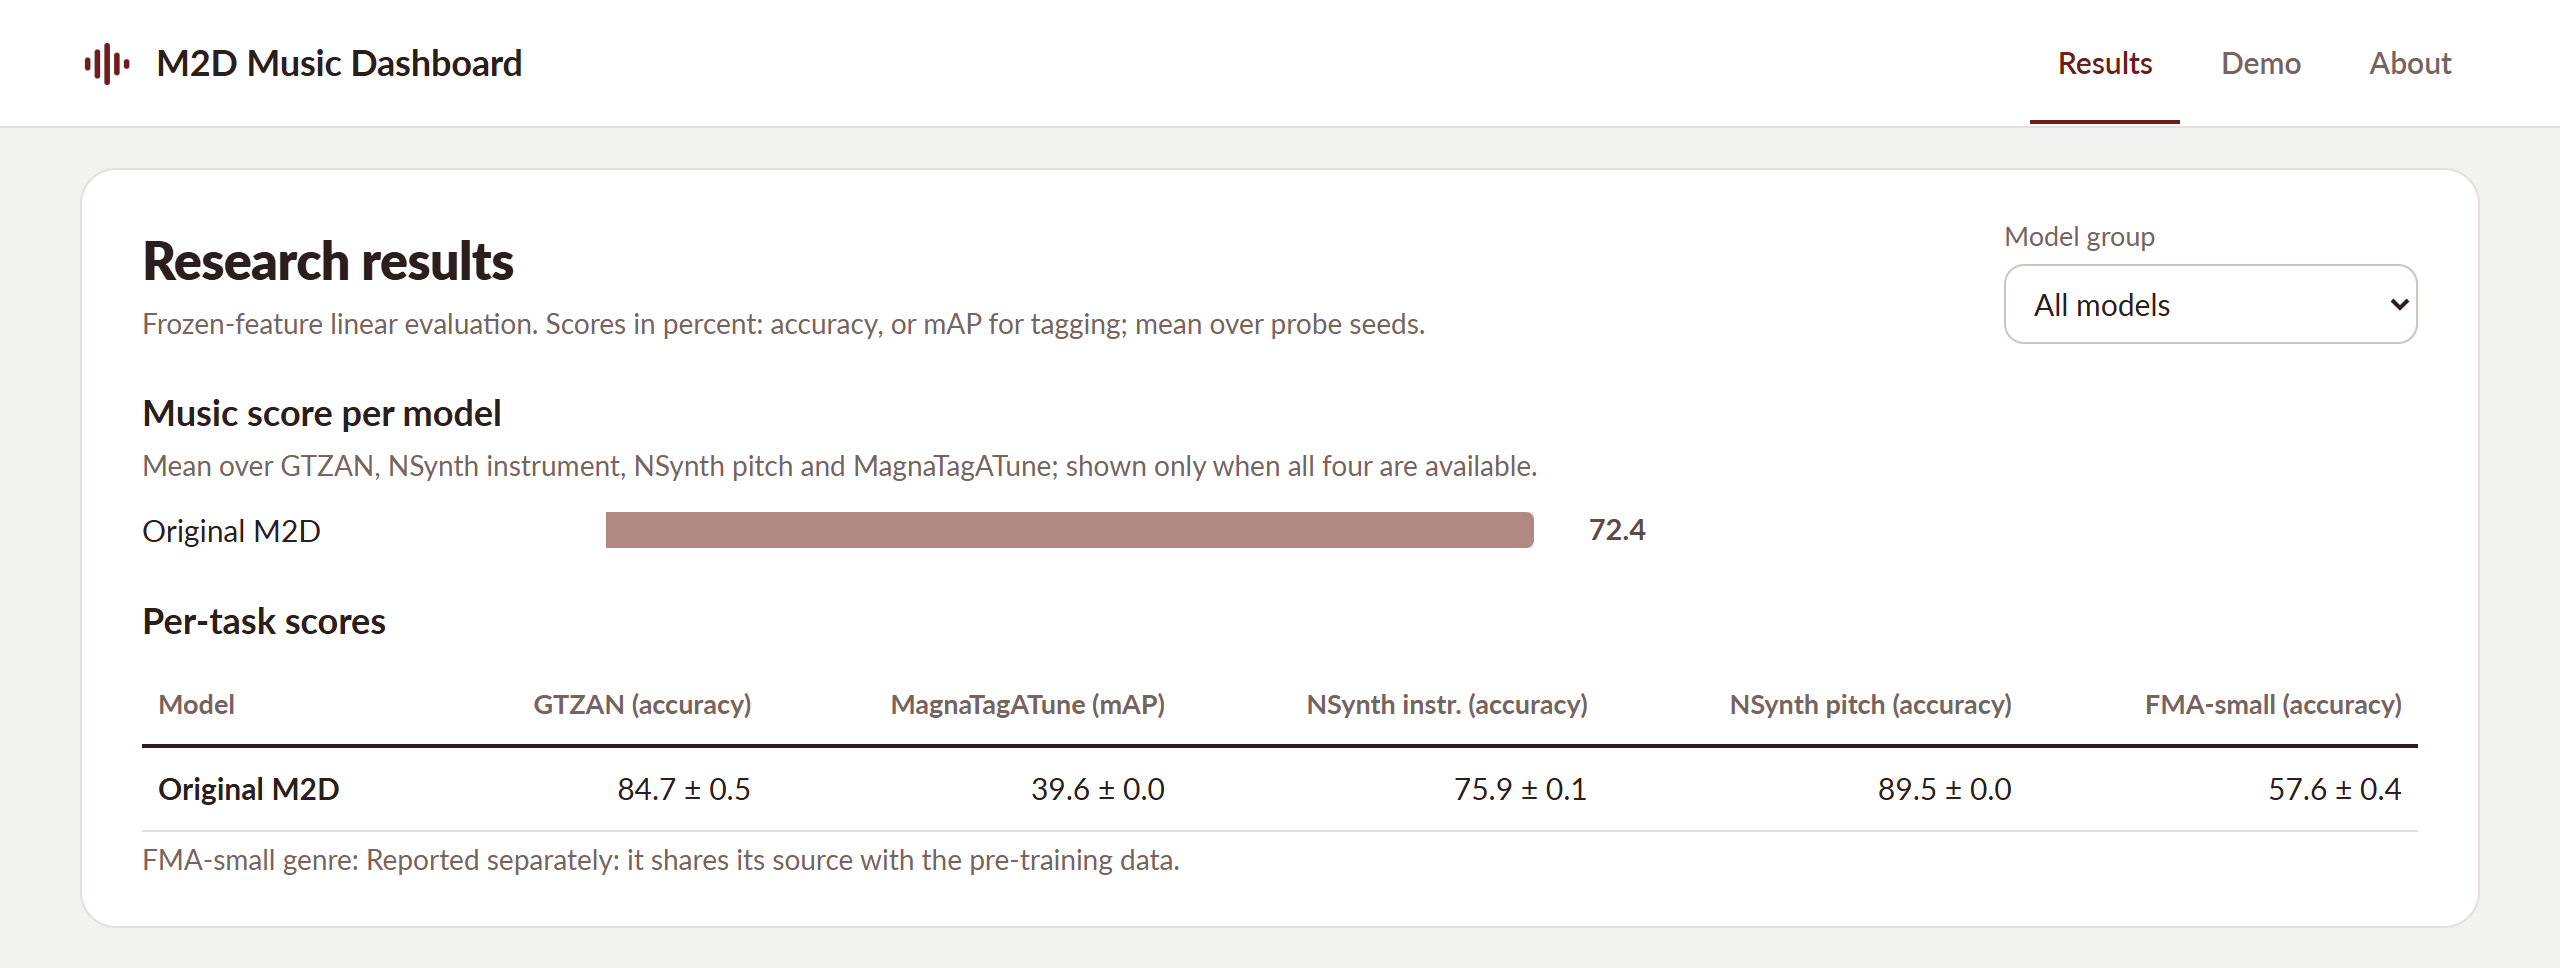
\includegraphics[width=\linewidth]{Figures/gui/gui_results.png}
\caption[Results tab of the dashboard]{Results tab of the implemented dashboard with the reproduced EVAR linear-probe scores of the original M2D (arm A0). Values are mean $\pm$ standard deviation over six probe seeds.}
\label{fig:impl-results}
\end{figure}

\begin{figure}[htbp]
\centering
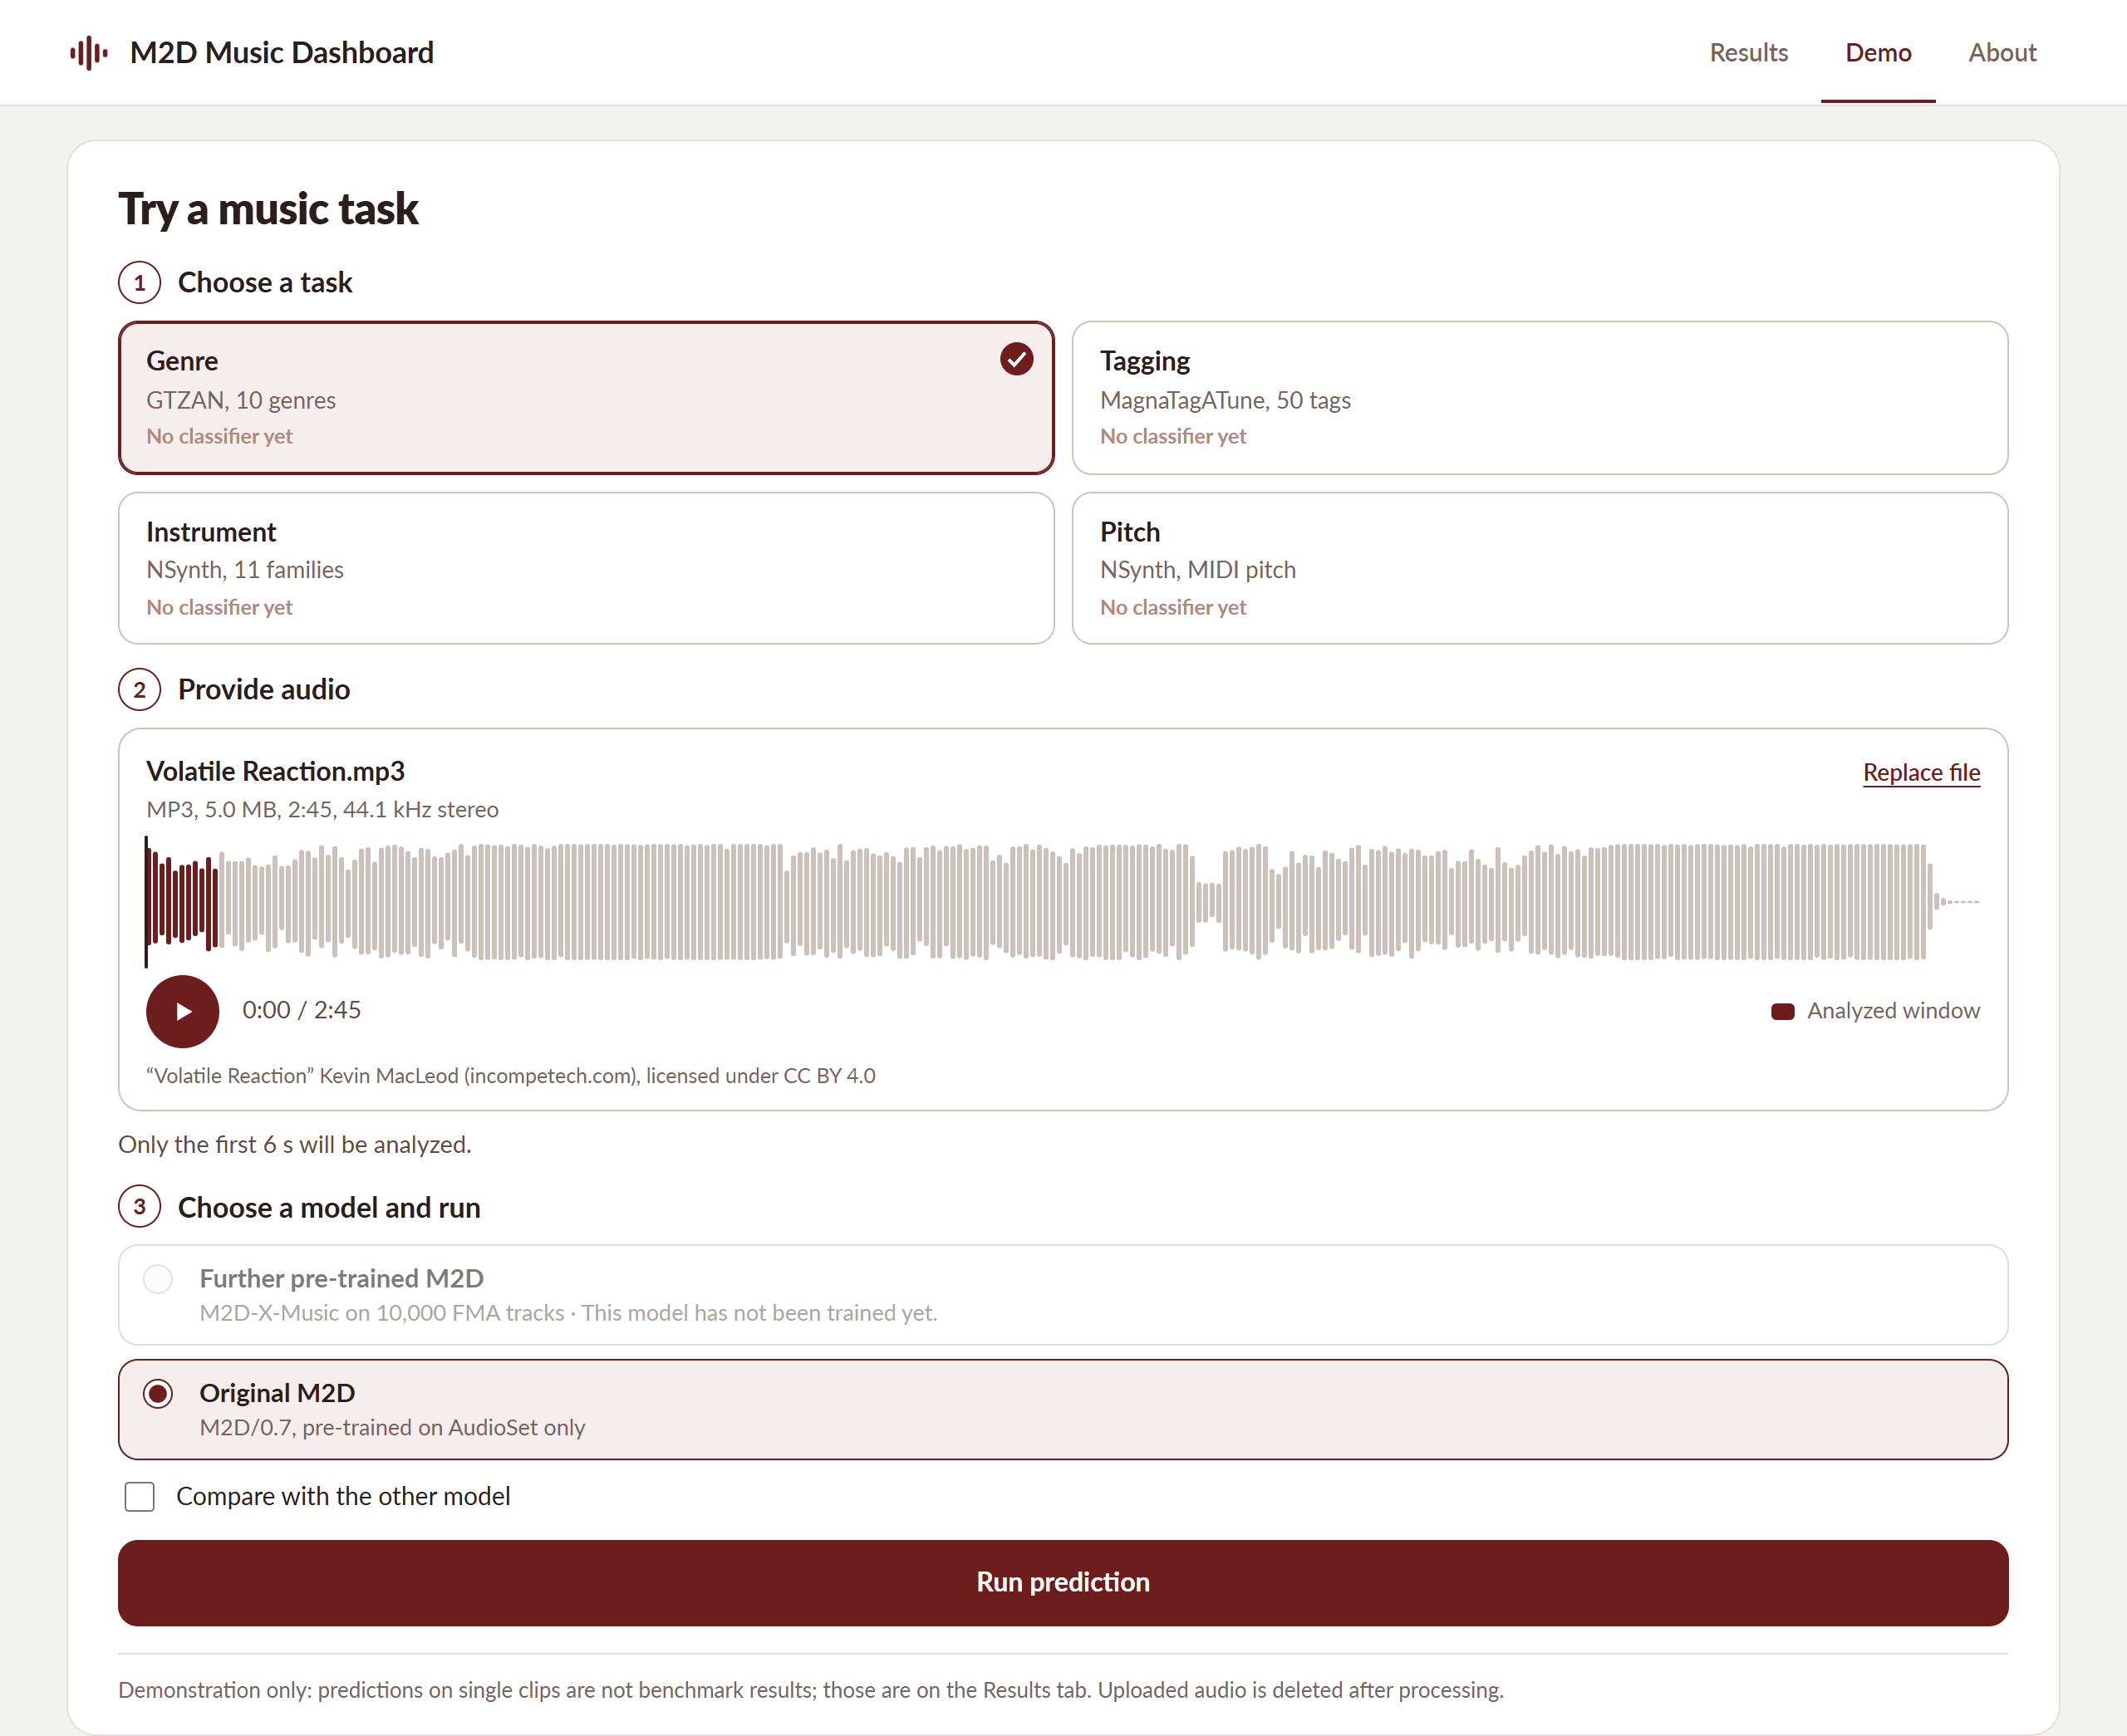
\includegraphics[width=0.92\linewidth]{Figures/gui/gui_form_clip.png}
\caption[Demo tab with a selected clip]{Demo tab with the bundled sample clip selected. The waveform marks the 6.08-s window that is analyzed, and tasks without a registered probe are labeled ``No classifier yet''.}
\label{fig:impl-demo}
\end{figure}

\begin{figure}[htbp]
\centering
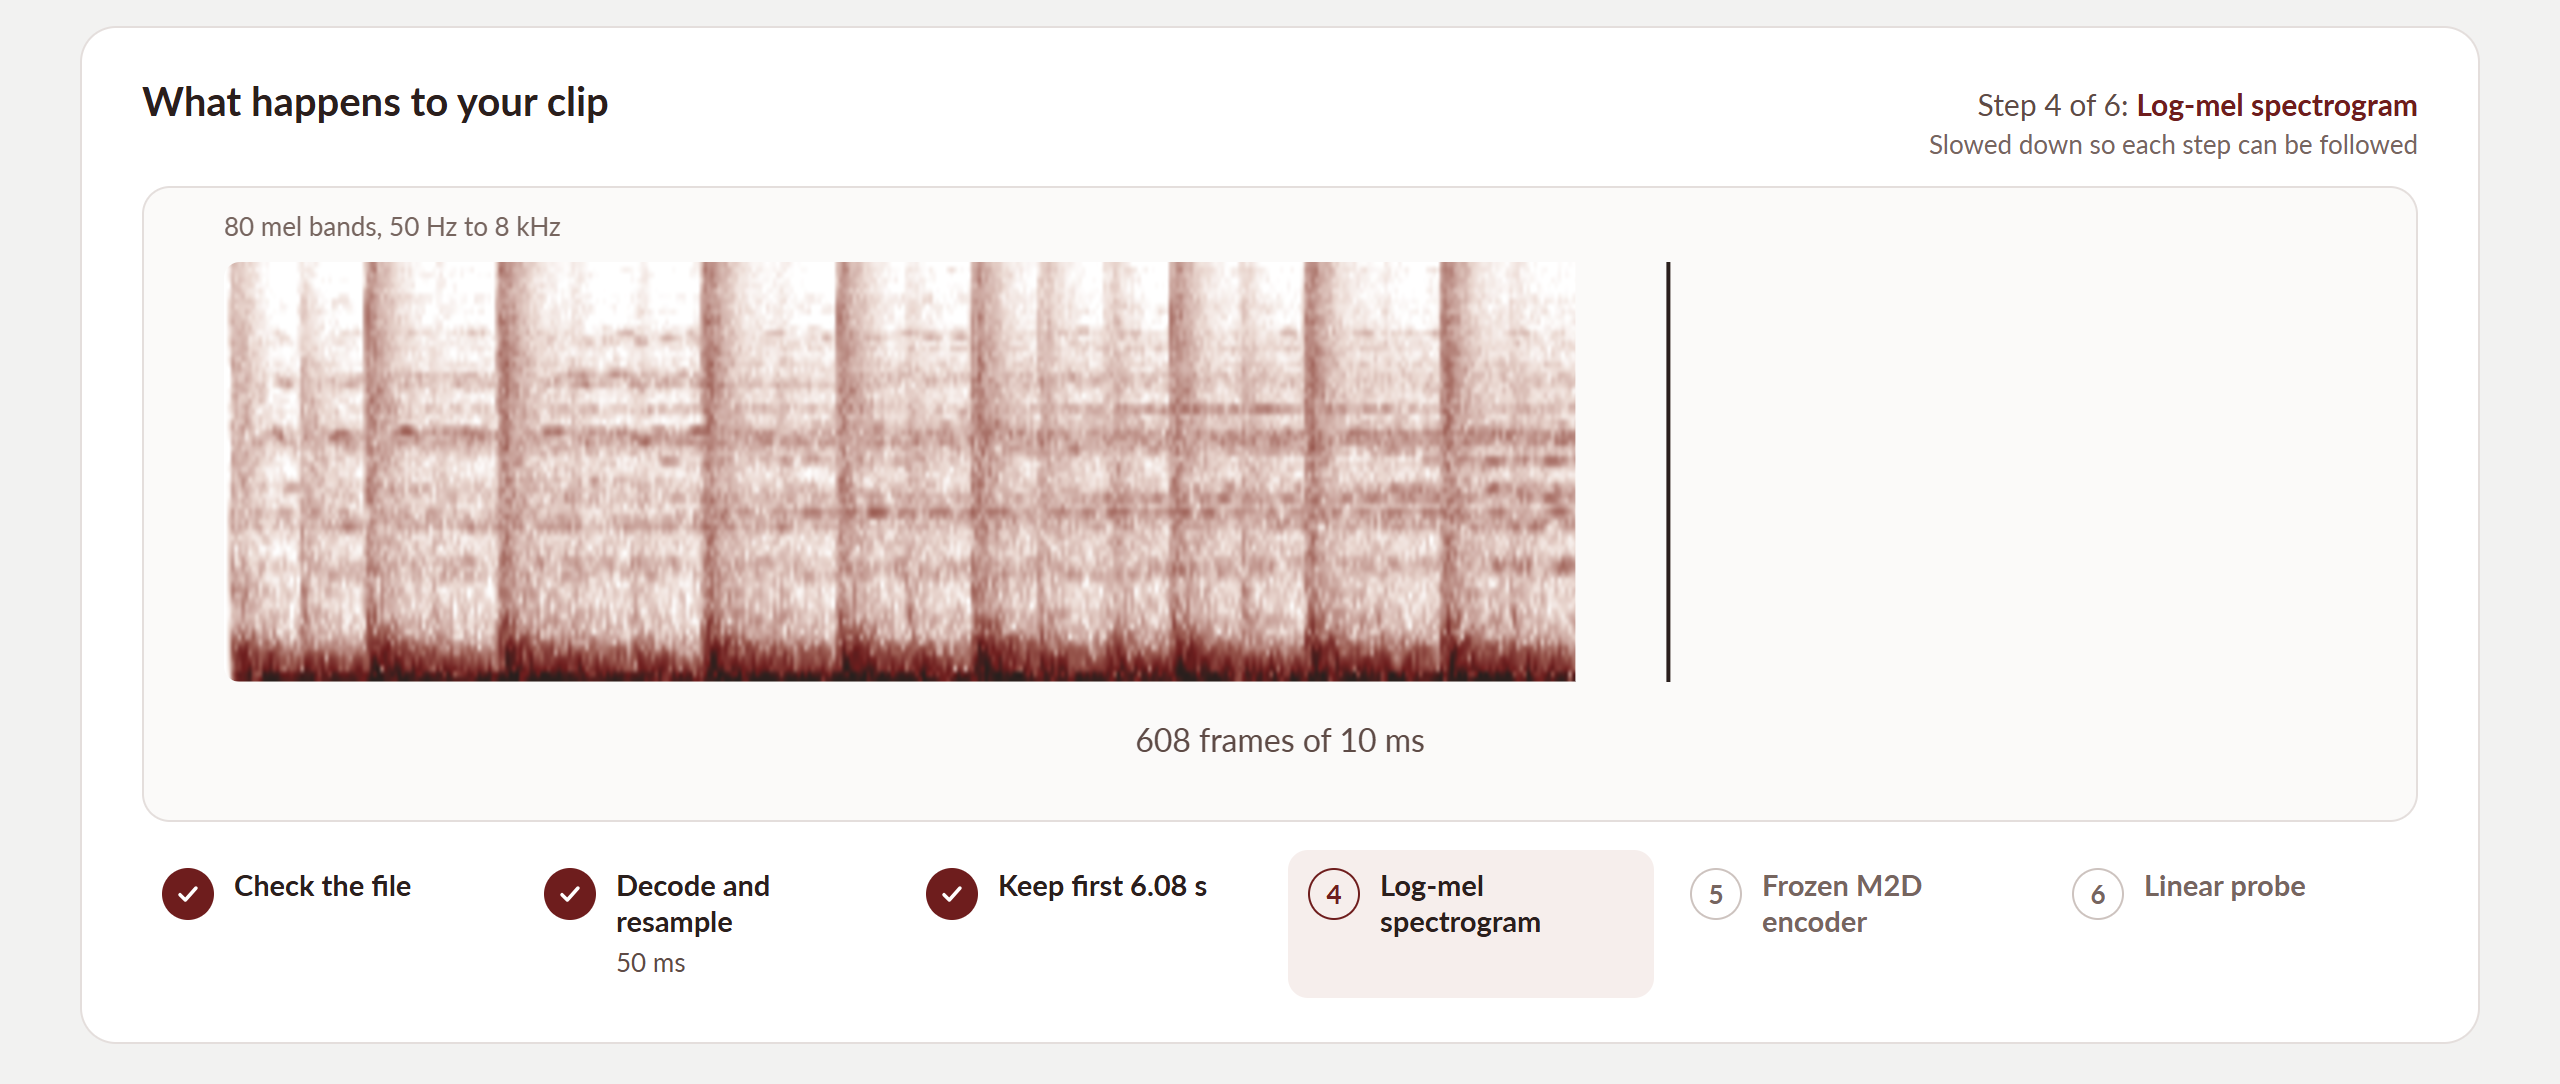
\includegraphics[width=\linewidth]{Figures/gui/gui_panel_running.png}
\caption[Pipeline animation during a prediction]{Pipeline animation during a prediction: the log-mel spectrogram of the analyzed window is drawn while the server computes the result. Completed steps show their measured time.}
\label{fig:impl-running}
\end{figure}

\begin{figure}[htbp]
\centering
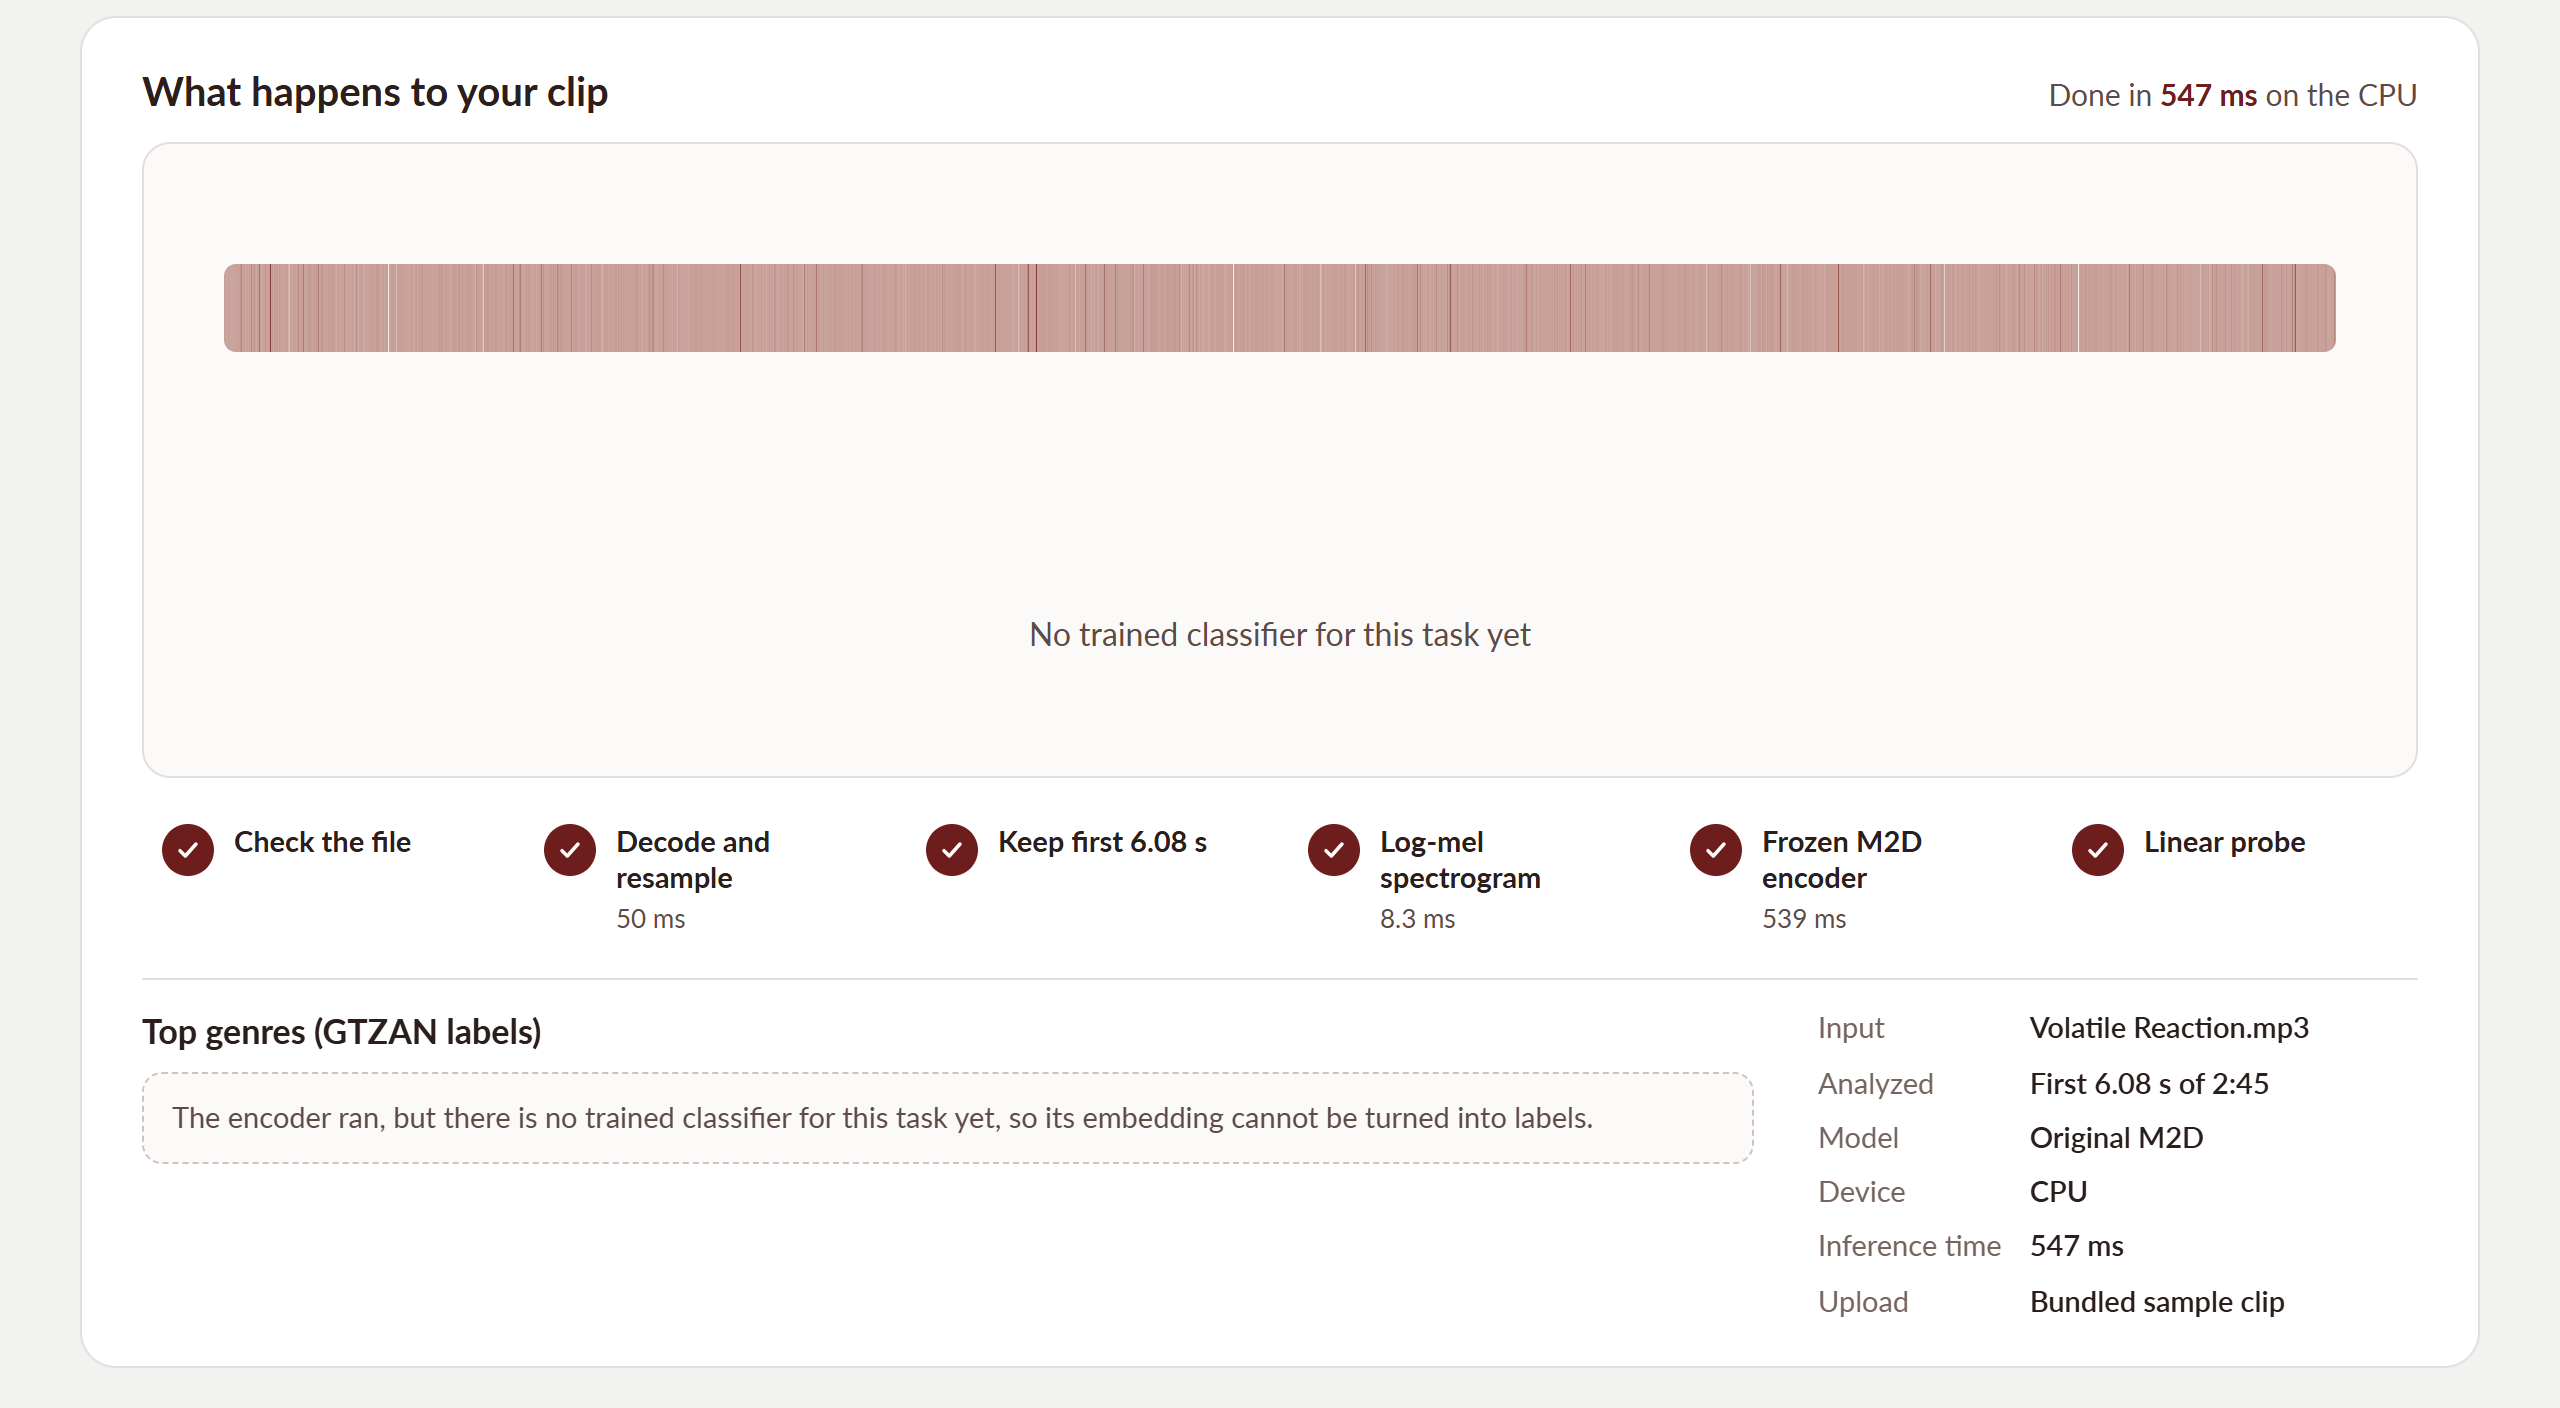
\includegraphics[width=\linewidth]{Figures/gui/gui_panel_output.png}
\caption[Output panel of a prediction]{Output panel after a prediction with the original M2D. The strip shows the real 3,840-dimensional embedding; because no probe is registered yet, the panel says so instead of showing scores.}
\label{fig:impl-output}
\end{figure}

\paragraph{Tools and libraries.} Table~\ref{tab:impl-tools} lists the tools used by the dashboard. The versions are those of the development environment.

\begin{table}[htbp]
\centering
\caption[Tools and libraries of the dashboard]{Tools and libraries of the dashboard.}
\label{tab:impl-tools}
\small\singlespacing
\begin{tabularx}{\linewidth}{>{\raggedright\arraybackslash}p{4.0cm}>{\raggedright\arraybackslash}p{2.2cm}Y}
\toprule
\textbf{Tool} & \textbf{Version} & \textbf{Use}\\
\midrule
Python & 3.12 & Language of the backend and scripts\\
PyTorch, torchaudio & 2.15 & Encoder inference and resampling\\
timm, einops, nnAudio & -- & Required by the M2D loader (ViT blocks and the log-mel front-end)\\
FastAPI, Uvicorn & 0.162 & Web API and server\\
SQLAlchemy, SQLite & 2.0 & Database access\\
soundfile & 0.12 or later & Decoding of WAV and MP3\\
pytest, httpx & -- & Automated tests and the API test client\\
HTML, CSS, JavaScript & -- & Frontend, without a framework or build step\\
Git and GitHub & -- & Version control; work is merged into \texttt{main} through pull requests\\
\bottomrule
\end{tabularx}
\end{table}

\section{Test case Design and description}
\label{sec:tests}
Testing covers the two components whose behavior can be checked at this stage: the dashboard and the evaluation pipeline. All test cases share the following attributes.
\begin{itemize}
  \item \textbf{Environment.} Unless stated otherwise, the tests run on a laptop with an Intel Core i5-8350U processor (four cores), 8~GB of memory, Windows~11, Python~3.12.4 and the CPU build of PyTorch~2.15. The browser tests use Microsoft Edge at a width of 1,280 pixels and, for the layout test, 390 pixels.
  \item \textbf{Inputs.} Audio inputs are either the bundled sample clip (``Volatile Reaction'', MP3, 165~s, 44.1~kHz stereo) or synthetic WAV files generated by the tests. No copyrighted dataset audio is used in the dashboard tests.
  \item \textbf{Shared dependencies.} The automated tests replace the encoder by a small fake model except in TC-07, which loads the real M2D/0.7 weights; this keeps the suite fast and lets it run without the 300~MB checkpoint.
  \item \textbf{Procedure.} Automated tests are run with \texttt{pytest}; manual tests follow the steps in their tables and are recorded with screenshots.
\end{itemize}
Table~\ref{tab:tc-summary} lists all test cases, and Tables~\ref{tab:tc-TC-01} to~\ref{tab:tc-TC-08} describe the main ones in the format of the template.

\begin{table}[htbp]
\centering
\caption[Summary of test cases]{Summary of test cases. A = automated (pytest), M = manual. All test cases were executed on 12 November 2026.}
\label{tab:tc-summary}
\small\singlespacing
\begin{tabularx}{\linewidth}{>{\raggedright\arraybackslash}p{1.1cm}>{\raggedright\arraybackslash}p{0.5cm}Y>{\raggedright\arraybackslash}p{2.3cm}>{\raggedright\arraybackslash}p{1.2cm}}
\toprule
\textbf{ID} & \textbf{Type} & \textbf{What is checked} & \textbf{Traces to} & \textbf{Result}\\
\midrule
TC-01 & A & Upload rules: allowed extensions and the 10~MB limit, checked by the server & FR-06, FR-08, UC-03 & Passed\\
TC-02 & A & Unsupported, unreadable and oversized files are rejected with a visitor-facing message & FR-08, UC-03 & Passed\\
TC-03 & A & The analysis window is exactly 6.08~s of 16~kHz mono audio; short clips are zero-padded; unreadable files give a message & FR-08, FR-09, FR-11 & Passed\\
TC-04 & A & A prediction on an upload returns the expected structure, and the uploaded file is deleted afterwards & FR-11, FR-12, FR-15, UC-04 & Passed\\
TC-05 & A & Without a probe, the system reports this honestly and invents no scores & FR-12, UC-04 & Passed\\
TC-06 & A & Probe storage, EVAR conversion, and refusal of MLP probes and of tagging probes without tag names & FR-12, FR-17 & Passed\\
TC-07 & A & The real M2D/0.7 encoder returns one finite 3,840-dimensional embedding per clip & FR-11 & Passed\\
TC-08 & A & Compare mode lists the untrained model as unavailable; the music score appears only with all four tasks; the group filter & FR-01, FR-03, FR-13, UC-05 & Passed\\
TC-09 & A & Health and catalogue endpoints: loaded models, the four demo tasks with their probe status, and the sample clip & FR-05, FR-07 & Passed\\
TC-10 & M & Importing a results CSV fills the Results tab; an invalid row aborts the whole import & FR-02, FR-17, UC-06 & Passed\\
TC-11 & M & Concurrent requests are queued and receive increasing queue positions & FR-14, NFR capacity & Passed\\
TC-12 & M & Prediction latency on CPU and loading time of the Results view & NFR performance & Passed\\
TC-13 & M & Layout at phone width has no horizontal scrolling & NFR compatibility & Passed\\
TC-14 & M & Baseline reproduction: A0 scores lie within the tolerance of the published M2D scores & Evaluation pipeline & Passed\\
\bottomrule
\end{tabularx}
\end{table}

\testcase{TC-01}{Upload validation}{UC-03; FR-06, FR-08}
{Verify that the server itself accepts only WAV and MP3 files of at most 10~MB, independently of the checks in the browser.}
{pytest with the FastAPI test client; fake encoder.}
{Backend installed; test database created by the test fixture.}
{\tcstep{1}{Call the upload check with a file named \texttt{a.MP3}.}{Accepted as MP3; the extension check ignores case.}
\tcstep{2}{Call the upload check with \texttt{a.flac}.}{Rejected with ``Unsupported file format''.}
\tcstep{3}{Call the upload check with a WAV file of 10~MB plus one byte.}{Rejected with ``File too large''.}}
{The size limit is also enforced while the file is received (TC-02).}
{Passed}

\testcase{TC-02}{Rejection of invalid files}{UC-03; FR-08}
{Verify that invalid uploads end with a clear message and leave no file behind.}
{pytest with the FastAPI test client; fake encoder.}
{Test app running with a temporary upload folder.}
{\tcstep{1}{POST a file named \texttt{a.flac}.}{HTTP 422 with ``Unsupported file format. Please use WAV or MP3.''; the upload folder is empty.}
\tcstep{2}{POST a file named \texttt{a.mp3} that contains non-audio bytes.}{HTTP 422 with ``The file could not be read.''; the upload folder is empty.}
\tcstep{3}{Lower the size limit to 1,000 bytes and POST a larger WAV file.}{HTTP 422 with ``File too large (maximum 10 MB).''}
\tcstep{4}{In the browser, choose a text file in the Demo tab.}{The message ``Unsupported file format. Please use WAV or MP3.'' appears under the drop zone (Figure~\ref{fig:man-error}).}}
{Steps 1--3 are automated; step 4 was checked by hand. Step 3 lowers the limit so that the test does not have to send 10~MB.}
{Passed}

\testcase{TC-03}{Analysis window}{UC-04; FR-09, FR-11}
{Verify that every input is turned into exactly one 6.08-s window of 16~kHz mono audio.}
{pytest; synthetic WAV files.}
{None.}
{\tcstep{1}{Load a 10-s stereo WAV file at 44.1~kHz.}{The window has 97,280 float32 samples; the input is reported as stereo at 44.1~kHz with a duration of 10~s; 6.08~s are analyzed and \texttt{padded} is false.}
\tcstep{2}{Load a 2-s mono WAV file at 16~kHz.}{\texttt{padded} is true, 2~s are analyzed, and all samples after the first 2~s are zero.}
\tcstep{3}{Load a file of non-audio bytes named \texttt{broken.mp3}.}{The loader raises the visitor message ``could not be read''.}}
{The 6.08-s length matches the 608-frame input of M2D/0.7.}
{Passed}

\testcase{TC-04}{Prediction and upload deletion}{UC-04; FR-11, FR-12, FR-15}
{Verify that a prediction on an uploaded file returns the documented response and that the uploaded file is deleted.}
{pytest with the FastAPI test client; fake encoder; a random linear probe registered for the genre task.}
{Probe file present in the temporary probe folder.}
{\tcstep{1}{POST an 8-s stereo WAV file with \texttt{task=genre} and \texttt{model=original}.}{HTTP 200; one result with status \texttt{ok}, ten genre scores that sum to one and the top-5 labels; the input is reported as stereo with 6.08~s analyzed.}
\tcstep{2}{List the upload folder.}{The folder is empty.}
\tcstep{3}{Read the inference log.}{Exactly one row, with status \texttt{ok} and source \texttt{upload}.}}
{Shows FR-15 and FR-16 together. The test log stores no file name or address by design of the table (Figure~\ref{fig:srs-er}).}
{Passed}

\testcase{TC-05}{Prediction without a probe}{UC-04; FR-12}
{Verify that the system never shows invented scores when no classifier has been trained for a task.}
{pytest with the FastAPI test client; fake encoder; a probe only for the genre task. Repeated by hand with the real encoder.}
{No probe registered for the tagging task.}
{\tcstep{1}{POST a WAV file with \texttt{task=tagging}, for which no probe is registered.}{Status \texttt{no\_probe}; an embedding is returned but no labels.}
\tcstep{2}{Run the same request in the browser.}{The output panel shows the embedding and the message that no classifier exists yet (Figure~\ref{fig:impl-output}).}}
{This is the current state of the deployed dashboard until the EVAR probes are exported.}
{Passed}

\testcase{TC-06}{Probe conversion}{UC-06; FR-12, FR-17}
{Verify that EVAR probe files are converted correctly and that unusable probes are refused.}
{pytest; synthetic EVAR files with a linear layer, a scaler and a label encoder.}
{None.}
{\tcstep{1}{Save a 10-class probe and load it again with safe loading; compute scores for a random embedding.}{Ten scores that sum to one; a 50-tag probe gives 50 sigmoid scores strictly between 0 and 1.}
\tcstep{2}{Convert a synthetic EVAR file with a linear layer, a scaler and a label encoder.}{The labels are blues, jazz and rock, the probe is single-label, and the stored mean equals the scaler mean.}
\tcstep{3}{Convert an EVAR file with a hidden layer, and a 50-output file without tag names.}{Both conversions stop with an error; with tag names given, the second file converts to a multi-label probe.}}
{Prevents a silent mismatch between dashboard and evaluation.}
{Passed}

\testcase{TC-07}{Real encoder}{UC-04; FR-11}
{Verify that the downloaded M2D/0.7 weights load with the official loader and produce one embedding per clip.}
{pytest; CPU; real checkpoint in the models folder (the test is skipped when the weights are absent).}
{Weights downloaded with \texttt{download\_models.py}.}
{\tcstep{1}{Load the checkpoint.}{All keys match; input size 80$\times$608; feature dimension 3,840.}
\tcstep{2}{Embed 6.08~s of noise.}{One vector of 3,840 finite values.}}
{Runs in about 20~s on the test laptop, most of it for loading the model.}
{Passed}

\testcase{TC-08}{Comparison and music score}{UC-01, UC-05; FR-01, FR-03, FR-13}
{Verify the compare mode and the rule that the music score is shown only when all four music tasks have results.}
{pytest with the FastAPI test client; fake encoder.}
{Results for some tasks imported into the test database.}
{\tcstep{1}{POST a prediction with \texttt{compare=true}.}{Two results: the original model with status \texttt{ok} and the further pre-trained model, which has no checkpoint, with status \texttt{model\_unavailable}.}
\tcstep{2}{Store scores of 80, 40, 70 and 90 for the four music tasks of the original model and a single score for MERT-v1-95M; request \texttt{/api/results}.}{The original model has a music score of 70.0; MERT-v1-95M, with one task only, has none.}
\tcstep{3}{Request \texttt{/api/results?group=reference}.}{Only MERT-v1-95M is listed.}}
{Step 3 also checks the model-group filter (FR-03).}
{Passed}

\section{Test Metrics}
\label{sec:test-metrics}
Table~\ref{tab:test-metrics} gives the metrics of the template for the test cases of Table~\ref{tab:tc-summary}. The automated suite consists of 16 pytest functions, some of which are parameterized, and the summary groups them into nine test cases; five further test cases were run by hand. All 14 test cases passed on 12 November 2026. Four defects were found during testing and fixed before this run: the per-task table of the Results tab stayed empty because a table header and body were appended in the wrong way; the probability bars had zero width in narrow table cells; the page was 459 pixels wide on a 375-pixel phone screen; and the Linux start script had Windows line endings and did not run. All four were found by the manual test cases, which gives a test case effectiveness of 100\,\% for the defects known so far.

\begin{table}[htbp]
\centering
\caption[Test metrics]{Test metrics of the dashboard and evaluation tests.}
\label{tab:test-metrics}
\small\singlespacing
\begin{tabularx}{\linewidth}{>{\raggedright\arraybackslash}p{4.6cm}>{\raggedright\arraybackslash}p{2.6cm}Y}
\toprule
\textbf{Metric} & \textbf{Value} & \textbf{Purpose}\\
\midrule
Number of test cases & 14 (9 automated, 5 manual) & Total number of test cases developed for the system\\
Number of test cases passed & 14 & Test cases that passed\\
Number of test cases failed & 0 & Test cases that failed\\
Test case defect density & 0\,\% & (Failed test cases $\times$ 100) / executed test cases\\
Test case effectiveness & 100\,\% (4 of 4) & (Defects found by test cases $\times$ 100) / all defects found\\
Requirement coverage & 17 of 18 FR & Share of functional requirements traced to at least one test case (Table~\ref{tab:test-trace})\\
\bottomrule
\end{tabularx}
\end{table}

\subsection{Traceability Matrix}
Table~\ref{tab:test-trace} links each functional requirement of Chapter~\ref{ch:srs} to the test cases that cover it. FR-18 (the About page) is checked only by inspection (Figure~\ref{fig:man-about}) and has no dedicated test case. FR-04 (the bar chart) is covered only for the original model, because no other model has results yet; it will be tested again when the results of the further pre-trained and reference models are imported in FYP-II.

\begin{table}[htbp]
\centering
\caption[Traceability matrix]{Traceability matrix between functional requirements and test cases.}
\label{tab:test-trace}
\small\singlespacing
\begin{tabular}{lll}
\toprule
\textbf{Requirement} & \textbf{Test cases} & \textbf{Status}\\
\midrule
FR-01 Results overview and music score & TC-08, TC-10 & Covered\\
FR-02 Per-task table & TC-10 & Covered\\
FR-03 Model-group filter & TC-08, TC-10 & Covered\\
FR-04 Bar chart & TC-10 & Partly (one model)\\
FR-05 List of tasks & TC-09 & Covered\\
FR-06 Upload & TC-01 & Covered\\
FR-07 Sample clip & TC-09, TC-05 & Covered\\
FR-08 Input checks & TC-01, TC-02 & Covered\\
FR-09 Mono, 16~kHz & TC-03 & Covered\\
FR-10 Model choice & TC-08 & Covered\\
FR-11 Frozen-encoder embedding & TC-03, TC-04, TC-07 & Covered\\
FR-12 Task output & TC-04, TC-05, TC-06 & Covered\\
FR-13 Comparison & TC-08 & Covered\\
FR-14 Queue & TC-11 & Covered\\
FR-15 Deletion of uploads & TC-02, TC-04 & Covered\\
FR-16 Anonymous log & TC-04 & Covered\\
FR-17 Developer import & TC-06, TC-10 & Covered\\
FR-18 About page & -- & Inspection only\\
\bottomrule
\end{tabular}
\end{table}

\section{Conclusion}
\label{sec:impl-conclusion}
FYP-I has produced three working components. The data pipeline has acquired and audited the corpora and converted them with the front-end of the original model. The evaluation pipeline implements both the EVAR linear protocol and the MARBLE probe, with seed and bootstrap intervals and an automatic check against published scores, and it has been run on the original M2D. The dashboard runs the real M2D encoder behind a small API, deletes uploads, queues requests and shows only results that exist. Fourteen test cases cover 17 of the 18 functional requirements and all passed after four defects had been fixed. What remains is the further pre-training itself, the export of the probes into the dashboard and the tests that depend on them, which are part of the plan for FYP-II.

% =====================================================================
\chapter{User Manual}
\label{ch:manual}
This chapter explains how to install, start and use the M2D Music Dashboard. It is written for two kinds of reader: a visitor, such as an evaluator or a student, who only opens the dashboard in a browser, and the developer, who installs it, adds probes and imports results. The manual describes version~1.0 of the dashboard as it stands at the end of FYP-I and will be updated in FYP-II when the further pre-trained model and its probes are added.

\section{Installation}
\label{sec:man-install}
The dashboard runs on Windows, Linux and macOS with Python~3.12. A GPU is optional; on a recent laptop CPU a prediction takes well under a second (Section~\ref{sec:res-dash}). The installation is done once.
\begin{enumerate}
  \item Clone the repository and open a terminal in its folder.
  \item Create a virtual environment:\\ \texttt{python -m venv .venv}
  \item Install PyTorch (the CPU build, or the CUDA build on a GPU machine) and the other packages:\\ \texttt{.venv/Scripts/pip install -r requirements.txt}\\ On Linux and macOS the folder is \texttt{.venv/bin} instead of \texttt{.venv/Scripts}.
  \item Download the M2D/0.7 weights and loader:\\ \texttt{.venv/Scripts/python backend/scripts/download\_models.py}\\ The files are placed in the user's cache folder and are not stored in the repository.
  \item Optionally, check the installation:\\ \texttt{.venv/Scripts/python -m pytest backend/tests}\\ All 16 tests should pass.
\end{enumerate}

\section{Starting and Stopping}
\label{sec:man-start}
On Windows, double-click \texttt{start.bat}; on Linux, run \texttt{./start.sh}. The script starts the server at \texttt{http://127.0.0.1:8000} and opens the browser. The server loads the models once, which takes a few seconds, and then prints \emph{Application startup complete}. To stop it, press Ctrl+C in the terminal. If port 8000 is already in use, start the server by hand on another port:\\ \texttt{.venv/Scripts/python -m uvicorn backend.app:app --port 8001}

\section{Using the Dashboard}
\label{sec:man-use}
The page has three tabs, Results, Demo and About, in the top bar (Figure~\ref{fig:impl-results}). Every tab can be reached from every other tab, and the browser's back button works between them.

\subsection{Viewing the Results}
The Results tab opens first. It shows the music score of each model as a bar and a table of the per-task scores, as mean $\pm$ standard deviation over the probe seeds. The \emph{Model group} menu at the top right restricts the view to the M2D models or to the reference models. FMA-small is shown in its own column and is not part of the music score, because it comes from the same source as the pre-training data; a note under the table says so. A model without results for all four music tasks has no bar.

\subsection{Running a Prediction}
The Demo tab guides the visitor through three numbered steps (Figure~\ref{fig:impl-demo}).
\begin{enumerate}
  \item \textbf{Choose a task.} Click one of the four task cards: Genre (GTZAN, 10 genres), Tagging (MagnaTagATune, 50 tags), Instrument (NSynth, 11 instrument families) or Pitch (NSynth, MIDI pitch). A card marked ``No classifier yet'' can be run, but it returns only the embedding.
  \item \textbf{Provide audio.} Drop a WAV or MP3 file of at most 10~MB on the drop zone, click \emph{Browse files}, or click the sample clip. The file card shows the name, format, size, length and sampling rate, and the waveform marks the first 6.08~s, which is the part that is analyzed. The play button plays the clip. \emph{Replace file} chooses another clip.
  \item \textbf{Choose a model and run.} Select the original or the further pre-trained M2D. A model that is not available yet is greyed out. Tick \emph{Compare with the other model} to run both models on the same clip. Click \emph{Run prediction}.
\end{enumerate}
While the server works, the panel \emph{What happens to your clip} shows the six steps of the pipeline: checking the file, decoding and resampling, keeping the first 6.08~s, computing the log-mel spectrogram, running the frozen encoder and applying the linear probe (Figure~\ref{fig:impl-running}). Completed steps show the time they took on the server. When the result arrives, the panel shows the embedding as a colored strip and the output of the task: the five most likely genres, instrument families or pitches, or the tags whose probability is above the threshold of 0.5. The table at the right gives the input, the analyzed part, the model, the device and the inference time (Figure~\ref{fig:impl-output}). In compare mode, the two outputs are shown side by side and labels that only one model predicts are highlighted.

\subsection{Messages and Errors}
Table~\ref{tab:man-messages} lists the messages that a visitor can see and what to do. Errors appear in red under the step that caused them (Figure~\ref{fig:man-error}).

\begin{table}[htbp]
\centering
\caption[Messages shown by the dashboard]{Messages shown by the dashboard and the action to take.}
\label{tab:man-messages}
\small\singlespacing
\begin{tabularx}{\linewidth}{>{\raggedright\arraybackslash}p{5.6cm}Y}
\toprule
\textbf{Message} & \textbf{Meaning and action}\\
\midrule
Unsupported file format. Please use WAV or MP3. & The file is of another type. Convert it to WAV or MP3.\\
File too large (maximum 10 MB). & Shorten the clip; only the first 6~s are used anyway.\\
The file could not be read. & The file is damaged or not really audio. Try another file.\\
No classifier yet & No probe has been trained for this task and model. The embedding is still shown.\\
This model has not been trained yet. & The further pre-trained checkpoint is not registered; use the original model.\\
Waiting in queue (position $n$) & Another prediction is running; the request starts automatically.\\
The server is not running (banner) & Start the server as described in Section~\ref{sec:man-start} and reload the page.\\
\bottomrule
\end{tabularx}
\end{table}

\begin{figure}[htbp]
\centering
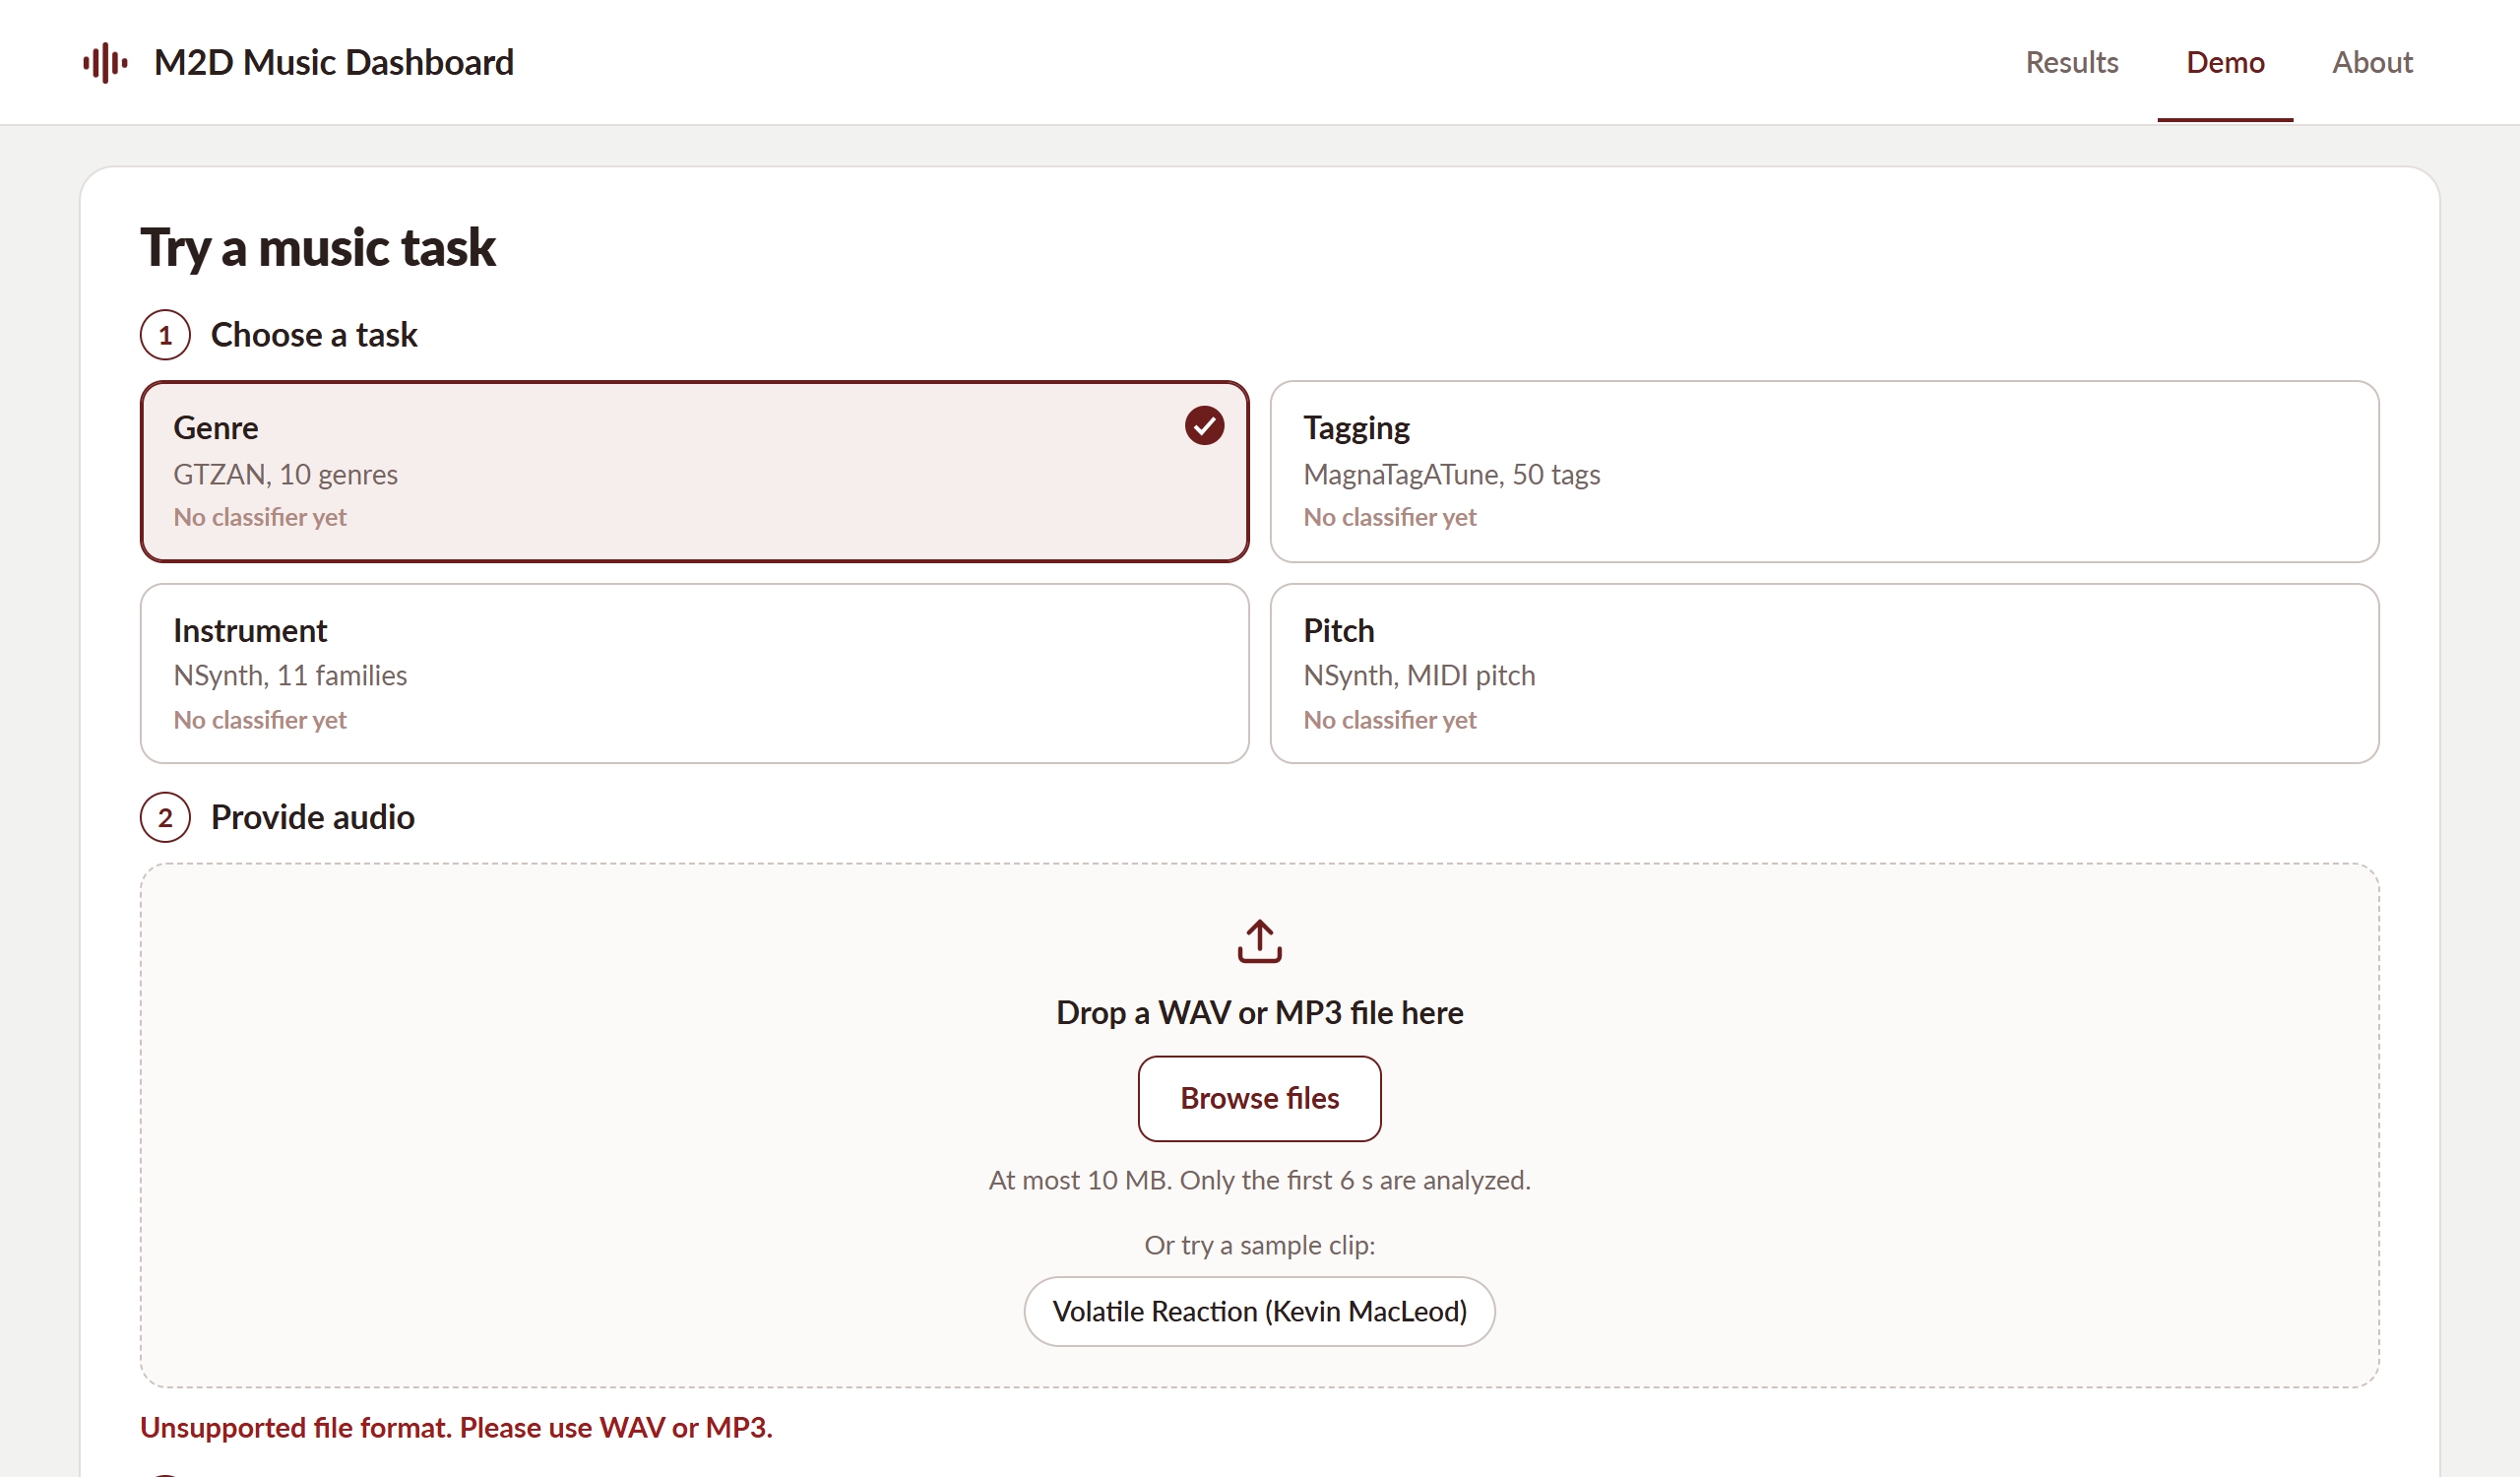
\includegraphics[width=0.85\linewidth]{Figures/gui/gui_form_error.png}
\caption[Error message for an unsupported file]{Error message after choosing a file of an unsupported type.}
\label{fig:man-error}
\end{figure}

\subsection{About Page}
The About tab describes the project, the method, the models and datasets, how the demonstration works, and the credits and licenses of the weights, the sample music and the font (Figure~\ref{fig:man-about}). It also states that a prediction on a single clip illustrates the models but does not show which one is better; the benchmark scores on the Results tab do that.

\begin{figure}[htbp]
\centering
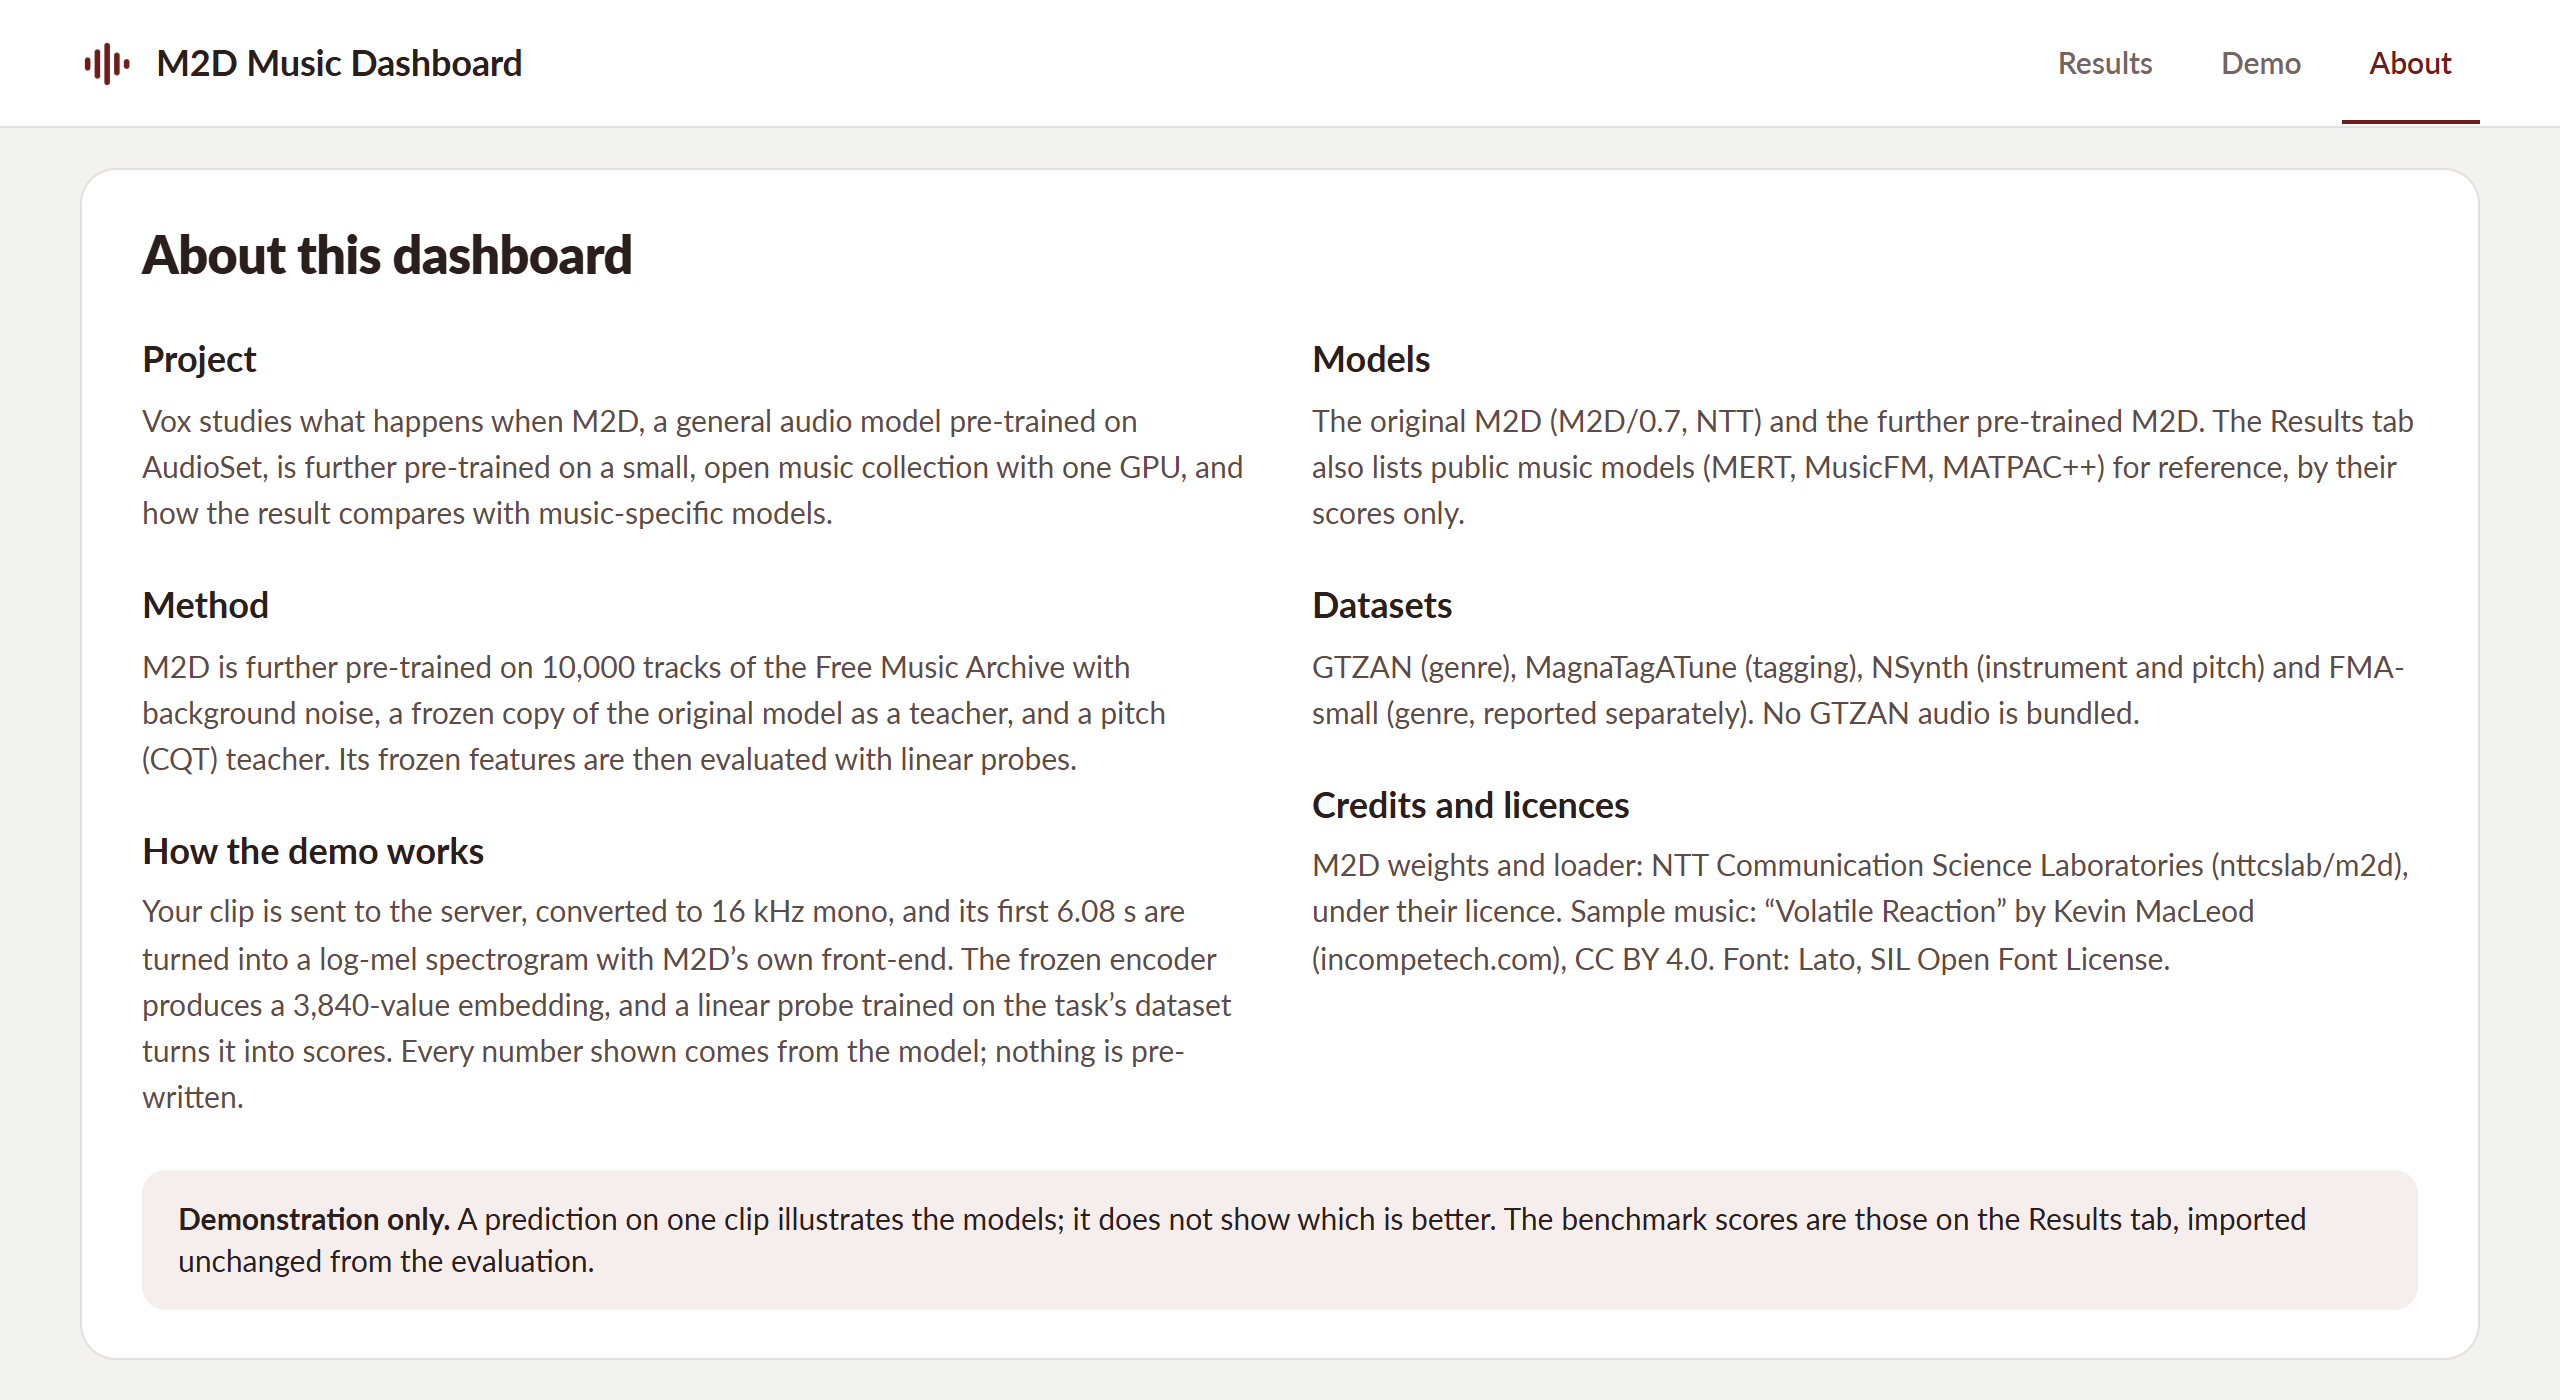
\includegraphics[width=\linewidth]{Figures/gui/gui_about.png}
\caption[About tab of the dashboard]{About tab of the dashboard.}
\label{fig:man-about}
\end{figure}

\section{Developer Tasks}
\label{sec:man-dev}
The developer maintains the dashboard with the script \texttt{backend/scripts/manage.py}. The web interface itself cannot change any data. Table~\ref{tab:man-commands} lists the commands. After registering probes or a checkpoint, restart the server so that it loads them.

\begin{table}[htbp]
\centering
\caption[Developer commands]{Developer commands of \texttt{manage.py}.}
\label{tab:man-commands}
\small\singlespacing
\begin{tabularx}{\linewidth}{>{\raggedright\arraybackslash}p{6.3cm}Y}
\toprule
\textbf{Command} & \textbf{Effect}\\
\midrule
\texttt{init} & Creates the database and fills in the models, tasks and sample clip\\
\texttt{register-probe --model M --task T --evar DIR [--labels F]} & Converts the probe that EVAR saved in \texttt{DIR} and registers it. For tagging, \texttt{F} is a text file with the 50 tag names in EVAR's order\\
\texttt{import-results FILE.csv} & Imports scores with the columns \texttt{model, task, mean, std, ci\_low, ci\_high, n\_seeds}. Every row is checked first, and nothing is imported if any row is invalid\\
\texttt{set-checkpoint --model further --path P} & Points the further pre-trained model at its checkpoint\\
\texttt{add-sample --code C --file F --title T ...} & Adds a sample clip with its license and attribution\\
\texttt{status} & Lists the models, checkpoints, probes, results and log size\\
\bottomrule
\end{tabularx}
\end{table}

To make the predictions of the original model real, the four probes are exported from EVAR by running its linear evaluation with saving switched on, for example \texttt{python lineareval.py config/m2d.yaml gtzan weight\_file=\ldots\ --save=True}, for GTZAN, NSynth instrument, NSynth pitch and MagnaTagATune, and each one is registered with \texttt{register-probe}.

\section{Conclusion}
\label{sec:man-conclusion}
The dashboard is installed with four commands, started with one script and used through three tabs without an account. A visitor can read the research results, run the four music tasks on a clip of their own or on the bundled sample, and follow each step of the prediction with its measured time. The developer adds probes, checkpoints and results with one script, and the interface cannot alter them. The manual will be extended in FYP-II with the comparison of the original and the further pre-trained model once both have probes.

% =====================================================================
\chapter{Experimental Results and Discussion}
\label{ch:results}
This chapter presents the experiments carried out during FYP-I. Following the guidance for this deliverable, it reports the experiments that have been completed and leaves the rest for FYP-II. Two experiments are reported. The first reproduces the published scores of the original M2D/0.7 model with our evaluation pipeline; this is arm A0 of the experimental design (Table~\ref{tab:m5-arms}) and the reference point against which every further pre-trained model will be compared. The second measures the response time of the dashboard against its non-functional requirements. The chapter closes with what these results imply for the experiments of FYP-II.

\section{Experimental Setup}
\label{sec:res-setup}
The original checkpoint \texttt{m2d\_vit\_base-80x608p16x16-221006-mr7} (epoch 300) was evaluated with frozen features on the five tasks of Table~\ref{tab:m5-tasks}, using the two probe protocols of Section~\ref{sec:impl-eval}: the EVAR linear probe with six seeds and the MARBLE probe (one hidden layer of 512 units) with five seeds. All scores are percentages: accuracy for GTZAN, NSynth instrument (NSynthI), NSynth pitch (NSynthP) and FMA-small, and mean average precision (mAP) for MagnaTagATune (MTT). Each score is reported as the mean over seeds with the half-width of the 95\,\% $t$-interval, together with the 95\,\% bootstrap interval over test clips. The music score $S_{\mathrm{mus}}$ is the mean of the primary scores of GTZAN, MTT, NSynthI and NSynthP (Equation~\ref{eq:m5-agg}); FMA-small is reported separately. A score counts as reproduced when it differs from the published value by at most twice the seed standard deviation plus 0.5 points.

\section{Reproduction of the Original M2D}
\label{sec:res-a0}
Table~\ref{tab:res-a0} gives the primary scores and Figure~\ref{fig:res-a0} compares them with the published values. Every score for which a published value exists was reproduced. With the EVAR linear probe, GTZAN reached 84.71\,\% against a published 84.1\,\% and NSynthI 75.86\,\% against 75.7\,\%. With the MARBLE probe, the differences were $-1.57$ points on GTZAN, $-0.01$ on MTT mAP, $+0.05$ on MTT ROC-AUC, $+0.22$ on NSynthI and $+0.02$ on NSynthP. The largest difference, on GTZAN, is well inside the tolerance because GTZAN has only 290 test clips and its scores vary by about one point between seeds. The music score of the original model is 72.43 with the linear probe and 72.04 with the MARBLE probe.

\begin{table}[htbp]
\centering
\caption[Reproduced scores of the original M2D (A0)]{Reproduced scores of the original M2D/0.7 (arm A0). Mean over probe seeds $\pm$ half-width of the 95\,\% $t$-interval, the 95\,\% bootstrap interval over test clips, and the published value where one exists. All values in percent.}
\label{tab:res-a0}
\small\singlespacing
\begin{tabular}{llcccc}
\toprule
\textbf{Protocol} & \textbf{Task (metric)} & \textbf{Mean $\pm$ CI} & \textbf{Bootstrap 95\,\%} & \textbf{Published} & \textbf{Reproduced}\\
\midrule
EVAR linear & GTZAN (acc.) & 84.71 $\pm$ 1.40 & 81.26--87.93 & 84.1 & yes\\
(6 seeds) & MTT (mAP) & 39.59 $\pm$ 0.07 & 38.90--41.05 & -- & --\\
 & NSynthI (acc.) & 75.86 $\pm$ 0.15 & 74.61--77.08 & 75.7 & yes\\
 & NSynthP (acc.) & 89.54 $\pm$ 0.11 & 88.71--90.38 & -- & --\\
 & FMA-small (acc.) & 57.62 $\pm$ 0.99 & 54.73--60.52 & -- & --\\
 & $S_{\mathrm{mus}}$ & 72.43 $\pm$ 0.33 & 71.56--73.46 & -- & --\\
\midrule
MARBLE MLP & GTZAN (acc.) & 79.93 $\pm$ 2.85 & 76.14--83.66 & 81.5 & yes\\
(5 seeds) & MTT (mAP) & 40.49 $\pm$ 0.22 & 39.81--41.92 & 40.5 & yes\\
 & MTT (ROC-AUC) & 91.45 $\pm$ 0.11 & 91.21--91.68 & 91.4 & yes\\
 & NSynthI (acc.) & 78.42 $\pm$ 1.04 & 77.31--79.54 & 78.2 & yes\\
 & NSynthP (acc.) & 89.32 $\pm$ 0.33 & 88.54--90.10 & 89.3 & yes\\
 & FMA-small (acc.) & 55.50 $\pm$ 2.04 & 52.88--58.05 & -- & --\\
 & $S_{\mathrm{mus}}$ & 72.04 $\pm$ 0.63 & 71.10--73.15 & -- & --\\
\bottomrule
\end{tabular}
\end{table}

\begin{figure}[htbp]
\centering
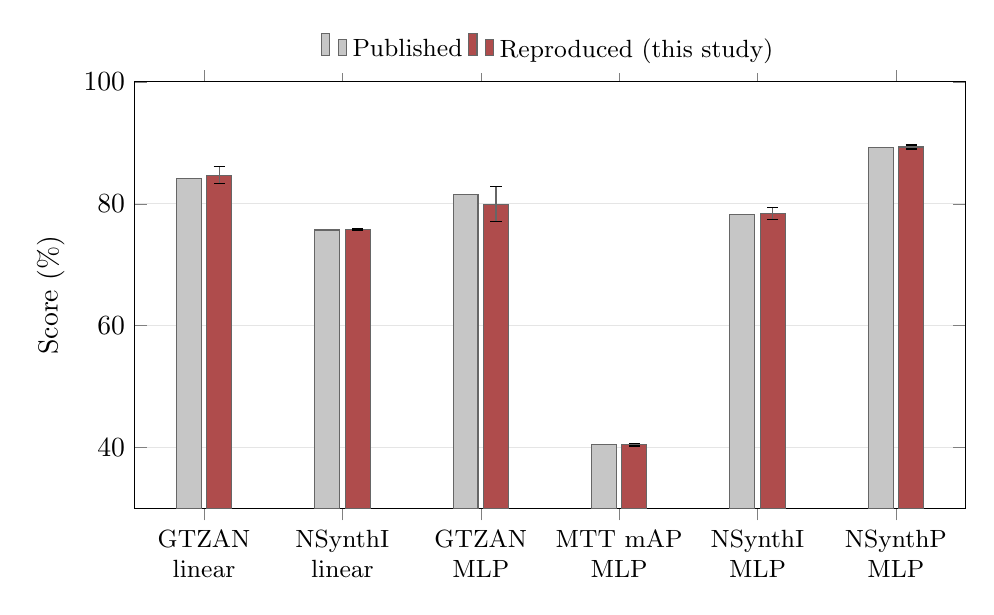
\begin{tikzpicture}
\begin{axis}[
  ybar, bar width=9pt, width=\linewidth, height=7cm,
  ymin=30, ymax=100, ylabel={Score (\%)},
  symbolic x coords={GTZAN-L,NSynthI-L,GTZAN-M,MTT-M,NSynthI-M,NSynthP-M},
  xticklabels={{GTZAN\\linear},{NSynthI\\linear},{GTZAN\\MLP},{MTT mAP\\MLP},{NSynthI\\MLP},{NSynthP\\MLP}},
  xtick=data, x tick label style={align=center, font=\small},
  legend style={at={(0.5,1.02)}, anchor=south, legend columns=2, font=\small, draw=none},
  enlarge x limits=0.1, ymajorgrids, grid style={black!10},
]
\addplot[fill=gray!45, draw=black!60] coordinates {(GTZAN-L,84.1) (NSynthI-L,75.7) (GTZAN-M,81.5) (MTT-M,40.5) (NSynthI-M,78.2) (NSynthP-M,89.3)};
\addplot[fill=red!55!black!70, draw=black!60, error bars/.cd, y dir=both, y explicit] coordinates {
  (GTZAN-L,84.71) +- (0,1.40) (NSynthI-L,75.86) +- (0,0.15) (GTZAN-M,79.93) +- (0,2.85)
  (MTT-M,40.49) +- (0,0.22) (NSynthI-M,78.42) +- (0,1.04) (NSynthP-M,89.32) +- (0,0.33)};
\legend{Published, Reproduced (this study)}
\end{axis}
\end{tikzpicture}
\caption[Published and reproduced scores of the original M2D]{Published and reproduced scores of the original M2D/0.7. Error bars show the 95\,\% $t$-interval over probe seeds.}
\label{fig:res-a0}
\end{figure}

\section{Discussion of the Baseline}
\label{sec:res-discussion}
\paragraph{The evaluation pipeline can be trusted.} Reproducing the published numbers was the first goal of the experiments, because every later claim is a difference from this baseline. An error in the front-end, in the window length or in the pooling would have shown up as a systematic gap of several points; instead, all seven comparable scores lie within the tolerance, five of them within a quarter of a point of the published values. The same pipeline, with the same seeds and splits, will now be applied to each further pre-trained checkpoint, so any change that FYP-II reports will come from the model and not from the measurement.

\paragraph{The two protocols disagree by task.} The music scores of the two protocols are almost equal (72.43 and 72.04), but the tasks behave differently. The linear probe is 4.8 points better on GTZAN, while the MLP probe is 2.6 points better on NSynthI and 0.9 points better on MTT mAP. GTZAN has only 443 training clips, too few to fit a hidden layer of 512 units reliably, and the MLP results on GTZAN also have twice the seed spread of the linear ones. NSynthI and MTT have tens of thousands of training examples, and there the extra capacity of the MLP can exploit structure that a linear layer cannot. For the main comparisons we therefore keep the linear probe of Section~\ref{sec:m5-eval}, which measures the frozen features most directly and matches the M2D papers, and we report the MARBLE probe as a secondary view that is comparable to the MARBLE literature.

\paragraph{Secondary metrics reveal class effects.} On NSynthP the accuracy is 89.5\,\% but the balanced accuracy is only 80.8\,\% (Table~\ref{tab:res-secondary}). Notes in the middle of the MIDI range are frequent and well recognized, whereas the rare very high and very low notes are often wrong, and accuracy hides this. On MTT, the macro F1 at a threshold of 0.5 is low (32.6 with the linear probe), because most of the 50 tags are rare and their probabilities seldom pass 0.5; mAP, which does not depend on a threshold, is the better primary metric here, as in MARBLE. These observations matter for FYP-II because the CQT teacher is meant to improve pitch: an improvement on the rare pitches would show up in the balanced accuracy before it shows up in the accuracy.

\begin{table}[htbp]
\centering
\caption[Secondary metrics of the original M2D]{Secondary metrics of the original M2D with the EVAR linear probe (six seeds), in percent.}
\label{tab:res-secondary}
\small\singlespacing
\begin{tabular}{lcccc}
\toprule
\textbf{Task} & \textbf{Accuracy / mAP} & \textbf{Balanced accuracy} & \textbf{Macro precision} & \textbf{Macro F1}\\
\midrule
GTZAN & 84.71 & 85.17 & 84.91 & 84.27\\
MTT & 39.59 (mAP) & -- & -- & 32.56\\
NSynthI & 75.86 & 76.56 & 70.37 & 69.28\\
NSynthP & 89.54 & 80.76 & 82.42 & 81.07\\
FMA-small & 57.62 & 57.62 & 57.33 & 57.23\\
\bottomrule
\end{tabular}
\end{table}

\paragraph{How large a gain can be detected.} The width of the bootstrap intervals sets the smallest change that FYP-II will be able to call supported. On GTZAN the interval spans about 6.7 points, so only a gain of several points could be supported on GTZAN alone; on NSynthI and NSynthP the intervals span about 2.5 and 1.7 points, and on MTT about 2.2 points. Because the paired bootstrap of Section~\ref{sec:m5-eval} compares two models on the same clips, it cancels much of the clip-to-clip variation and will be more sensitive than these unpaired intervals suggest, but the numbers show that GTZAN alone cannot carry a conclusion. This supports the decision to judge the arms by the music score and to treat GTZAN results with caution.

\paragraph{FMA-small as the in-domain check.} The original model reaches 57.6\,\% on FMA-small, far below its scores on the other genre task. FMA-small has eight broad genres with an artist filter, and its audio comes from the same archive as our pre-training data, so it is the task on which further pre-training is most likely to help. It is reported separately for exactly this reason: a gain on FMA-small alone would show adaptation to the archive rather than better music features in general.

\section{Performance of the Dashboard}
\label{sec:res-dash}
The dashboard was measured on the CPU of the test laptop (Intel Core i5-8350U, four threads for PyTorch) with the bundled MP3 clip, 30 sequential requests after two warm-up requests. Table~\ref{tab:res-latency} gives the times measured by the server. The median total inference time was 604~ms, of which almost all was spent in the encoder; the 90th percentile was 753~ms and the slowest request took 1.2~s. This is far below the target of 30~s on the CPU in Chapter~\ref{ch:srs}, and the target of 5~s on the GPU host will be met with a wide margin. The Results data were returned in 12 to 26~ms, against a target of 2~s for loading the view, and the server was ready about five seconds after it was started, against a target of two minutes. When four requests were sent at the same time, they received the queue positions 0, 1, 2 and 3 and were processed one after another, as required.

\begin{table}[htbp]
\centering
\caption[Response times of the dashboard on CPU]{Response times of the dashboard on CPU, in milliseconds, over 30 requests with the bundled MP3 clip.}
\label{tab:res-latency}
\small\singlespacing
\begin{tabular}{lcccc}
\toprule
\textbf{Stage} & \textbf{Median} & \textbf{Mean} & \textbf{90th percentile} & \textbf{Maximum}\\
\midrule
Decoding and resampling (MP3, 6.08~s kept) & 44.9 & 48.4 & 61.3 & 98.1\\
Log-mel spectrogram & 7.7 & 8.4 & 11.3 & 19.7\\
M2D encoder & 594.1 & 631.9 & 742.8 & 1198.0\\
Total inference (log-mel + encoder + probe) & 604.1 & 640.3 & 753.4 & 1217.7\\
\bottomrule
\end{tabular}
\end{table}

\section{Conclusion}
\label{sec:res-conclusion}
The evaluation pipeline reproduces every published score of the original M2D/0.7 within the tolerance, with a music score of 72.43 under the linear protocol and 72.04 under the MARBLE probe, and it gives the baseline A0 together with its uncertainty. The analysis shows that GTZAN is too small to decide a comparison on its own, that pitch accuracy hides weak performance on rare notes, and that FMA-small is the in-domain task where gains are most likely and must be interpreted with care. The dashboard answers in about 0.6~s on a laptop CPU, far within its targets. The further pre-training arms, the data-size study and the comparison with the music-specific reference models will be added to this chapter in FYP-II.

% =====================================================================
\chapter{Conclusions}
\label{ch:conclusions}
This chapter sums up the work of FYP-I, states how far the objectives have been met, describes the main challenges, and sets out the plan for FYP-II.

\section{Summary of the Work}
\label{sec:concl-summary}
The project asks whether a general-audio model can be made better at music cheaply, by further pre-training the AudioSet model M2D on 10,000 open FMA tracks on one GPU instead of training a music model from scratch. The literature review showed that music-specific models rely on large and often private collections and large compute budgets, that general-audio models such as M2D are already strong on music but weaker on pitch, and that further pre-training on a small dataset risks forgetting, which the M2D-X recipe counters with background noise and a frozen teacher. From this we derived M2D-X-Music, which adds a CQT musical teacher to M2D-X, and a set of compute-matched arms that switch one component at a time, evaluated with frozen features on music tasks. The requirements and design of a small demonstration dashboard were specified, together with the architecture of the whole research platform.

During FYP-I the data were acquired, audited and converted, the evaluation pipeline was built and validated by reproducing every published score of the original M2D, and the dashboard was implemented and tested. The baseline gives a music score of 72.43 with the linear protocol, and its intervals show how large a change the later comparisons can detect.

\section{Objectives Met and Not Yet Met}
\label{sec:concl-objectives}
Table~\ref{tab:concl-objectives} compares the state of the work with the objectives of Chapter~\ref{ch:vision}. The objectives that do not depend on further pre-training are met; those that compare further pre-trained models are planned for FYP-II, as foreseen in the project timeline.

\begin{table}[htbp]
\centering
\caption[Status of the objectives]{Status of the objectives at the end of FYP-I.}
\label{tab:concl-objectives}
\small\singlespacing
\begin{tabularx}{\linewidth}{Y>{\raggedright\arraybackslash}p{2.4cm}>{\raggedright\arraybackslash}p{4.4cm}}
\toprule
\textbf{Objective} & \textbf{Status} & \textbf{Evidence}\\
\midrule
Review the related work and identify the gap & Met & Chapter~\ref{ch:lr}\\
Prepare an audited, seeded pre-training corpus and noise corpus & Met & Section~\ref{sec:impl-data}\\
Build an evaluation pipeline and reproduce the original M2D & Met & Sections~\ref{sec:impl-eval} and~\ref{sec:res-a0}\\
Specify, design and build the demonstration dashboard & Met (v1.0) & Chapters~\ref{ch:srs}, \ref{ch:design} and Section~\ref{sec:impl-dash}\\
Implement the M2D-X-Music framework & In progress & Section~\ref{sec:impl-train}\\
Run arms A1--A5 and the data-size runs S1--S3 & Planned (FYP-II) & Section~\ref{sec:concl-plan}\\
Compare with the music-specific reference models & Planned (FYP-II) & Section~\ref{sec:concl-plan}\\
Answer the research questions & Planned (FYP-II) & --\\
\bottomrule
\end{tabularx}
\end{table}

\section{Challenges}
\label{sec:concl-challenges}
The main challenges so far were practical. The datasets are large and come in different formats, so the audit and conversion had to be resumable and had to record every rejected file. Matching the front-end of the original model exactly was essential, because a small difference in the spectrogram would have been confused with the effect of further pre-training; the successful reproduction of the published scores is the evidence that this was achieved. Published numbers use two different probe protocols, so both had to be implemented to check our pipeline against the literature. Finally, the compute budget of one 16~GB GPU limits the number of arms and seeds; the arms have therefore been ordered by importance so that the most informative ones run first.

\section{Future Work}
\label{sec:concl-future}
Beyond FYP-II, three directions follow from the design. A second pre-training seed for the best arms would separate the effect of the method from the randomness of a single run. The distillation of frozen MERT features as a second teacher would test whether a learned musical teacher helps more than the hand-crafted CQT. Finally, a version of the dashboard that runs the encoder in the browser would remove the need for a server during demonstrations.

\section{Plan for FYP-II}
\label{sec:concl-plan}
Table~\ref{tab:concl-plan} gives the plan for FYP-II. The arms are run in the priority order of Section~\ref{sec:m5-design}, so that the comparisons that answer the research questions are available first even if time runs short. Figure~\ref{fig:concl-gantt} shows the same plan as a timeline.

\begin{table}[htbp]
\centering
\caption[Plan for FYP-II]{Plan of the work for FYP-II.}
\label{tab:concl-plan}
\small\singlespacing
\begin{tabularx}{\linewidth}{>{\raggedright\arraybackslash}p{0.6cm}Y>{\raggedright\arraybackslash}p{2.6cm}>{\raggedright\arraybackslash}p{3.0cm}}
\toprule
\textbf{No.} & \textbf{Task} & \textbf{Period} & \textbf{Output}\\
\midrule
1 & Finish and test the M2D-X-Music extension (zero-CQT equivalence test, view-routing test); pilot run of one epoch & December 2026 & Tested training code, pilot log\\
2 & Further pre-training of A3 (M2D-X) and A1 (naive continuation) & December 2026 -- January 2027 & Two checkpoints\\
3 & Further pre-training of A4 (M2D-X-Music), A2 (noise only) and A5 (CQT without regularizer) & January -- February 2027 & Three checkpoints\\
4 & Evaluate every checkpoint with both protocols; paired bootstrap tests and gap-closure ratios & After each run & Updated Chapter~\ref{ch:results}\\
5 & Evaluate the reference models MERT-v1-95M, MERT-v0-public, MusicFM (FMA) and MATPAC++ & February 2027 & Reference scores\\
6 & Data-size runs S1--S3 with the best arm A$^{*}$ & March 2027 & Data-size curve\\
7 & Export the probes into the dashboard, register the best checkpoint, import all results; test FR-03, FR-04 and FR-13 with real models & March -- April 2027 & Dashboard v2.0\\
8 & Answer the research questions; optional runs if time remains & April 2027 & Discussion\\
9 & Final report, user manual update, demonstration and a paper draft & April -- May 2027 & Final deliverables\\
\bottomrule
\end{tabularx}
\end{table}

\begin{figure}[htbp]
\centering
\begin{tikzpicture}[x=1.7cm, y=0.62cm, font=\small]
  \foreach \m [count=\i from 0] in {Dec,Jan,Feb,Mar,Apr,May} {
    \node[anchor=south] at (\i+0.5, 0.2) {\m};
    \draw[black!15] (\i,0) -- (\i,-9.4);
  }
  \draw[black!15] (6,0) -- (6,-9.4);
  \newcommand{\gbar}[5]{\node[anchor=east, text width=4.6cm, align=right] at (-0.1,-#1+0.45) {#2};
    \fill[#5, rounded corners=1.5pt] (#3,-#1+0.15) rectangle (#4,-#1+0.75);}
  \gbar{1}{1. Finish code, pilot run}{0}{0.6}{blue!45}
  \gbar{2}{2. Arms A3 and A1}{0.5}{1.6}{orange!70}
  \gbar{3}{3. Arms A4, A2, A5}{1.4}{2.8}{orange!70}
  \gbar{4}{4. Evaluation and tests}{0.9}{4.3}{green!50!black!45}
  \gbar{5}{5. Reference models}{2.0}{2.9}{green!50!black!45}
  \gbar{6}{6. Data-size runs S1--S3}{2.8}{3.8}{orange!70}
  \gbar{7}{7. Dashboard v2.0}{3.0}{4.6}{blue!45}
  \gbar{8}{8. Research questions}{3.8}{4.8}{red!45}
  \gbar{9}{9. Final report and demo}{4.0}{6.0}{red!45}
\end{tikzpicture}
\caption[Timeline of FYP-II]{Timeline of FYP-II. Orange bars are training runs, green bars evaluation, blue bars software work and red bars analysis and writing.}
\label{fig:concl-gantt}
\end{figure}

\section{Conclusion}
\label{sec:concl-conclusion}
FYP-I has put in place everything that the experiments need: the data, a validated evaluation pipeline, a reproduced baseline with known uncertainty, and a working demonstration dashboard. The remaining work is the further pre-training itself and its analysis, which the plan for FYP-II schedules in order of importance. If the further pre-trained models improve on the baseline of 72.43, the project will have shown a low-cost route to better music representations; if they do not, the controlled arms will show which component failed and why, which is equally useful to others with a single GPU.
